% Informe del TP6: Mediciones en medios de comunicación analógicos y digitales.
\documentclass[12pt]{article}
\usepackage[utf8]{inputenc}
\usepackage[T1]{fontenc}
\usepackage{graphicx}
\usepackage[spanish,es-tabla,es-nodecimaldot]{babel}
\usepackage{amsmath}
\usepackage{amssymb}
\usepackage[a4paper,margin=1in]{geometry}
\usepackage{subcaption}
\usepackage{mathtools}
\usepackage[table,xcdraw]{xcolor}
\usepackage[style=ieee, backend=bibtex]{biblatex}
\usepackage{enumitem}
\usepackage{array}
\usepackage{longtable}
\usepackage{multirow}
\usepackage{booktabs}
\usepackage{csquotes}
\usepackage{tikz}
\usetikzlibrary{arrows.meta, positioning, shapes.geometric, fit, babel}
\usepackage[hidelinks]{hyperref}
\usepackage{float}
\usepackage{setspace}
\onehalfspacing
\graphicspath{{Figuras/}}

\addbibresource{bibliografia.bib}
\hypersetup{colorlinks=true, linkcolor=blue, citecolor=blue, urlcolor=blue, filecolor=blue}

% Datos que se completan después de las mediciones de laboratorio (se ven en rojo).
\newcommand{\pendiente}[1]{\textcolor{red}{[#1]}}

\begin{document}
\renewcommand{\figureautorefname}{Fig.}
\renewcommand{\tableautorefname}{Tab.}
\renewcommand{\equationautorefname}{Ec.}

\begin{titlepage}
\thispagestyle{empty}
\begin{tikzpicture}[remember picture,overlay]
    \node[opacity=0.2,anchor=center] at (current page.center)
        {
\includegraphics[width=0.9\paperwidth]{decoracion_a.png}};
\end{tikzpicture}
\begin{center}
    
\includegraphics[width=15cm]{unc_fcefyn_logo.png} \\ [0.5cm]
    \LARGE Universidad Nacional de Córdoba \\ [0.5cm]
    \large Facultad de Ciencias Exactas, Físicas y Naturales \\
    \vspace{40pt}
    \large Sistemas de Radiocomunicación \\ [0.2cm]
    \large Trabajo Práctico N.° 6 \\
    \vspace{50pt}
    \LARGE Medios \\[0.3cm]
    \large Mediciones en medios de comunicación analógicos y digitales \\
    \vspace{40pt}
    \begin{table}[!h]
        \centering
        \begin{tabular}{ll}
            \multicolumn{1}{c}{Nombre} & \multicolumn{1}{c}{DNI} \\
            Arteaga Barrera, Cristian Eduardo & 95.159.096 \\
            Baccino, Luca & 45.328.380 \\
            Mendes Rosa, Agustín & 44.517.201 \\
            Monja, Ernesto Joaquín & 43.873.728 \\
        \end{tabular}
    \end{table}
    \vspace{20pt}
    \begin{table}[!h]
        \centering
        \begin{tabular}{ll}
            \multicolumn{1}{c}{Docentes} & Esp. Ing. Liendo, Carlos Guillermo \\
                                         & Ing. Dadam, Federico Tomás \\
        \end{tabular}
    \end{table}
    \vfill
        {\small Comisión: \pendiente{completar} \quad Fecha de las mediciones: \pendiente{completar}\\[0.2cm]
         Córdoba, República Argentina\\ Año 2026}
\end{center}
\end{titlepage}

\newpage
\tableofcontents
\newpage
\listoffigures
\listoftables
\newpage

\section{Introducción}
\label{sec:introduccion}

El presente informe desarrolla la Actividad 6 de Sistemas de Radiocomunicación \cite{consigna}, dedicada a los medios de comunicación analógicos y digitales. La actividad tiene tres partes:
\begin{itemize}
    \item \underline{Parte 1:} mediciones con el analizador de espectro sobre señales recibidas de radiodifusión en AM, en FM, de televisión analógica y de televisión digital terrestre (TDA, norma ISDB-Tb). Para cada servicio se identifica la emisora o el canal con el Cuadro de Atribución de Bandas de Frecuencias de la República Argentina (CABFRA) \cite{cabfra}, se estima el ancho de banda ocupado y se interpreta el espectro según la modulación utilizada.
    \item \underline{Parte 2:} interpretación de los niveles expresados en dBm, dBµV y dBc, conversión entre ellos para sistemas de $50$ y $75 \, [\Omega]$, y cálculo del índice de modulación de una señal AM a partir de los niveles de portadora y de banda lateral.
    \item \underline{Parte 3:} investigación de las tecnologías que se usan para distribuir televisión y datos por cable y por fibra óptica: DVB-C, DOCSIS, Video RF Overlay en redes FTTH, ISDB-Tb e ISDB-Tb sobre cable.
\end{itemize}

La base teórica proviene de los videos de la asignatura \cite{videos_medios} y de la bibliografía de comunicaciones \cite{tomasi, haykin}. Los temas de la Parte 3 se apoyan en las normas de cada sistema y en documentación de fabricantes, que se citan en cada caso.

\subsection{Objetivos}
\begin{itemize}
    \item Utilizar el analizador de espectro para identificar y medir señales de radiofrecuencia, registrando en cada caso su configuración.
    \item Reconocer las características espectrales de las emisiones de AM, de FM y de televisión analógica y digital, y relacionarlas con la modulación y con la canalización de cada servicio.
    \item Interpretar los niveles de señal expresados en dBm, dBµV y dBc, y convertirlos entre sí teniendo en cuenta la impedancia.
    \item Describir las principales tecnologías de distribución de televisión y datos por redes de cable y de fibra óptica, con mayor detalle en el Video RF Overlay sobre FTTH, que complementa el diseño de la red FTTH del Trabajo Práctico 4 \cite{tp4}.
\end{itemize}

\section{Equipamiento y procedimiento}
\label{sec:equipamiento}

\subsection{Equipamiento utilizado}
En la \autoref{tab:equipamiento} se listan los instrumentos y elementos utilizados en las mediciones.

\begin{table}[H]
    \centering
    \caption{Equipamiento utilizado en las mediciones.}
    \label{tab:equipamiento}
    \begin{tabular}{p{4.2cm} p{4.6cm} p{5.6cm}}
        \toprule
        \textbf{Elemento} & \textbf{Marca y modelo} & \textbf{Características relevantes} \\
        \midrule
        Analizador de espectro & \pendiente{completar} & Rango de frecuencias, impedancia de entrada ($50 \, [\Omega]$), nivel máximo de entrada \\
        Bloqueador de continua (DC block) & \pendiente{completar} & Protege la entrada del analizador de tensiones continuas, por ejemplo la alimentación de un preamplificador de antena \\
        Antena para AM & \pendiente{completar} & \pendiente{tipo: hilo largo, cuadro o varilla} \\
        Antena para FM y TV & \pendiente{completar} & \pendiente{tipo: dipolo, Yagi o log-periódica; impedancia} \\
        Cables y conectores & \pendiente{completar} & \pendiente{tipo de cable (RG-58, RG-6), conectores BNC, N o F} \\
        Adaptador de impedancia & \pendiente{si se usó} & Adaptador de $75$ a $50 \, [\Omega]$ \\
        Televisor o receptor ISDB-Tb & \pendiente{completar} & Búsqueda automática de canales \\
        Osciloscopio & \pendiente{si se usó} & \\
        \bottomrule
    \end{tabular}
\end{table}

\subsection{Procedimiento}
\begin{enumerate}
    \item Se identificaron en el CABFRA \cite{cabfra} las bandas, los canales y las frecuencias de cada servicio, resumidos en la \autoref{tab:canalizacion}.
    \item Se conectó la antena correspondiente al analizador de espectro a través del bloqueador de continua, como se muestra en la \autoref{fig:conexion}. Solo se midieron señales recibidas: en ningún caso se conectó la salida de un transmisor al analizador.
    \item Antes de cada medición se configuró el instrumento y se registraron la frecuencia central o las de inicio y fin, el \textit{span}, el nivel de referencia, el ancho de banda de resolución (RBW), el ancho de banda de video (VBW), la atenuación, la preamplificación, la unidad y la impedancia de entrada.
    \item Se partió de los ajustes recomendados por la cátedra (nivel de referencia de $-30 \, [dBm]$, ganancia de $5$ a $10 \, [dB]$, RBW de $9 \, [kHz]$ y VBW de $100 \, [kHz]$) y se adaptaron a cada señal. Para explorar una banda completa conviene un RBW amplio, y para resolver la estructura de una emisión hace falta un RBW menor que los detalles que se quieren ver: las bandas laterales de AM, por ejemplo, requieren un RBW de $1 \, [kHz]$ o menos \cite{keysight_sa}.
    \item Se tomaron capturas de pantalla de cada medición, en las que se leen la señal y los parámetros, y fotografías de la antena, de los instrumentos y de las conexiones.
\end{enumerate}

\begin{table}[H]
    \centering
    \caption{Canalización de los servicios medidos según el CABFRA \cite{cabfra}.}
    \label{tab:canalizacion}
    \begin{tabular}{p{3.6cm} p{3.4cm} p{3.0cm} p{4.4cm}}
        \toprule
        \textbf{Servicio} & \textbf{Banda} & \textbf{Canalización} & \textbf{Observaciones} \\
        \midrule
        Radiodifusión sonora AM & $535$ a $1.605 \, [kHz]$ & 107 canales de $10 \, [kHz]$ & Se extiende con 10 canales más hasta $1.705 \, [kHz]$ (plan de Río de Janeiro, 1988) \\
        Radiodifusión sonora FM & $88$ a $108 \, [MHz]$ & Canales 201 a 300, de $200 \, [kHz]$ & El canal 201 está centrado en $88{,}1 \, [MHz]$ \\
        Televisión VHF baja & $54$ a $72$ y $76$ a $88 \, [MHz]$ & Canales 2 a 6, de $6 \, [MHz]$ & \\
        Televisión VHF alta & $174$ a $216 \, [MHz]$ & Canales 7 a 13, de $6 \, [MHz]$ & \\
        Televisión UHF & $470$ a $608$ y $614$ a $698 \, [MHz]$ & Canales 14 a 36 y 38 a 51, de $6 \, [MHz]$ & El canal 37 queda reservado a radioastronomía; la TDA usa esta banda \\
        \bottomrule
    \end{tabular}
\end{table}

El canal $N$ de FM está centrado en
\begin{equation}
    f_{FM}(N) = 88{,}1 \, [MHz] + 0{,}2 \, [MHz] \cdot (N - 201)
    \label{eq:canal_fm}
\end{equation}
y el canal UHF $N$ de televisión ocupa de $470 + 6\,(N-14)$ a $476 + 6\,(N-14) \, [MHz]$. En ISDB-Tb la portadora central se desplaza $1/7 \, [MHz]$ por encima del centro del canal, de modo que
\begin{equation}
    f_{ISDB}(N) = 473 + 6\,(N - 14) + \frac{1}{7} \, [MHz]
    \label{eq:canal_isdb}
\end{equation}

\begin{figure}[H]
    \centering
    \begin{tikzpicture}[node distance=1.6cm, every node/.style={font=\small},
        caja/.style={draw, rounded corners, minimum height=1cm, minimum width=2.4cm, align=center, fill=blue!6}]
        \node[caja] (ant) {Antena};
        \node[caja, right=of ant] (adap) {Adaptador\\$75/50 \, \Omega$\\(si corresponde)};
        \node[caja, right=of adap] (dc) {Bloqueador\\de continua};
        \node[caja, right=of dc, fill=orange!12] (sa) {Analizador\\de espectro\\$50 \, \Omega$};
        \draw[-{Stealth}] (ant) -- node[above]{coaxial} (adap);
        \draw[-{Stealth}] (adap) -- (dc);
        \draw[-{Stealth}] (dc) -- (sa);
    \end{tikzpicture}
    \caption{Conexión de la antena al analizador de espectro.}
    \label{fig:conexion}
\end{figure}

\begin{figure}[H]
    \centering
    \pendiente{Fotografía de la antena, de los instrumentos y de las conexiones (\texttt{Figuras/mediciones/montaje.jpg})}
    \caption{Montaje utilizado en el laboratorio.}
    \label{fig:montaje}
\end{figure}

\subsection{Impedancia y desadaptación}
El analizador de espectro tiene una entrada de $50 \, [\Omega]$, mientras que las antenas de televisión, los cables RG-6 y los receptores de radiodifusión trabajan normalmente en $75 \, [\Omega]$. Conectarlos directamente produce un coeficiente de reflexión
\begin{equation}
    \Gamma = \frac{Z_L - Z_0}{Z_L + Z_0} = \frac{50 - 75}{50 + 75} = -0{,}2
\end{equation}
y una pérdida por desadaptación de
\begin{equation}
    L_{des} = -10 \log\left(1 - |\Gamma|^2\right) = -10 \log(0{,}96) = 0{,}18 \, [dB]
\end{equation}
que es despreciable frente a la incertidumbre del resto de la medición. Un adaptador de mínima pérdida hace la transición sin reflexiones, pero introduce una atenuación conocida de unos $5{,}7 \, [dB]$ que debe sumarse a la lectura. En las mediciones \pendiente{se usó / no se usó} adaptador.

\newpage
\part*{Parte 1: Mediciones con analizador de espectro}
\addcontentsline{toc}{part}{Parte 1: Mediciones con analizador de espectro}
\section{Radiodifusión en AM}
\label{sec:am}

\subsection{Modulación AM}
En la modulación de amplitud con doble banda lateral y portadora completa, la envolvente de la portadora sigue a la señal modulante. Para un tono de frecuencia $f_m$ y un índice de modulación $m$, se cumple:
\begin{equation}
    v_{AM} = E_c \left[1 + m \cos(2\pi f_m t)\right] \cos(2\pi f_c t)
    = E_c \cos(2\pi f_c t) + \frac{m E_c}{2} \cos\left[2\pi (f_c \pm f_m) t\right]
    \label{eq:am}
\end{equation}

El espectro tiene tres componentes (\autoref{fig:am_teoria}, izquierda): 
\begin{itemize}
    \item \underline{La portadora}, en $f_c$, con amplitud $E_c$. No depende de la modulación y concentra al menos dos tercios de la potencia, aun con $m = 1$.
    \item \underline{Las bandas laterales inferior y superior}, en $f_c - f_m$ y $f_c + f_m$, con amplitud $m E_c / 2$ cada una. Llevan la información y son imágenes especulares una de la otra, es decir, hay una simetría exacta entre las dos bandas laterales.
\end{itemize}
En dBc (decibelios relativos a la portadora), cada banda lateral queda $20 \log(2/m)$ por debajo de la portadora: $6 \, [dB]$ con $m = 1$ y $12 \, [dB]$ con $m = 0{,}5$. Con una señal AM el resultado es un espectro continuo y simétrico alrededor de la portadora, que ocupa $2 f_{m,max}$ (\autoref{fig:am_teoria}, derecha).

\begin{figure}[H]
    \centering
    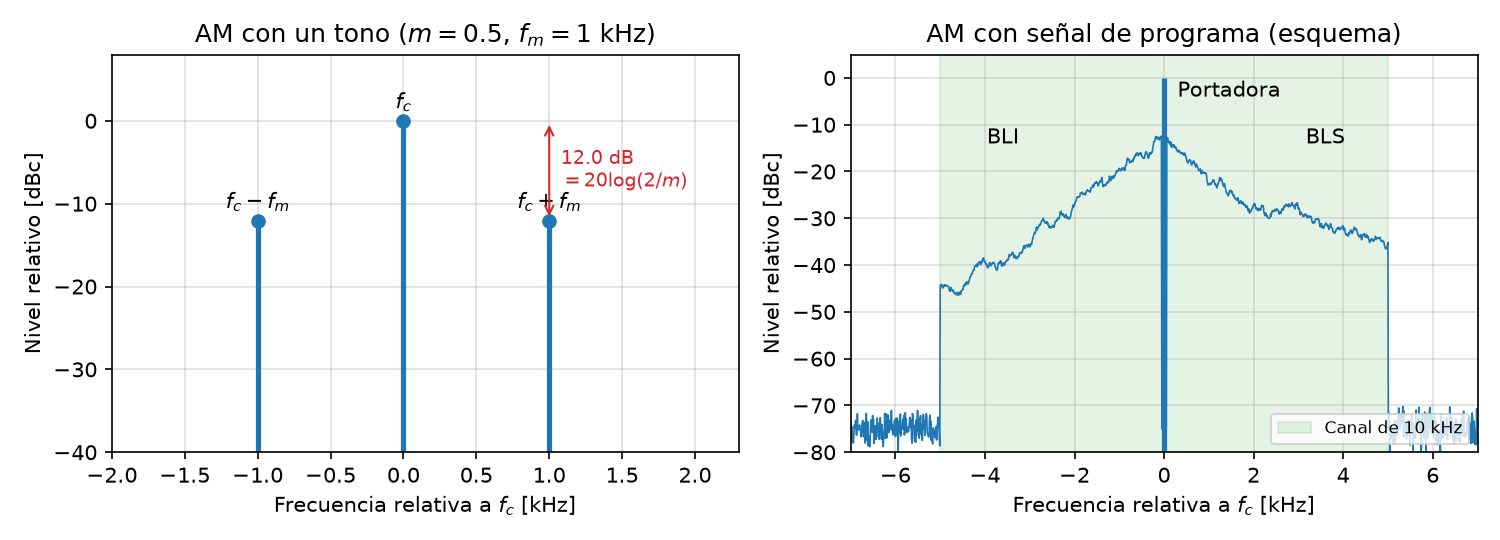
\includegraphics[width=\textwidth]{teoria/am_espectro.png}
    \caption{Espectro de AM con un tono (esquemas propios).}
    \label{fig:am_teoria}
\end{figure}

\subsection{Mediciones}

\subsubsection*{Exploración de la banda e identificación de las emisoras}
Se exploró la banda de radiodifusión en AM, que se extiende de $535$ a $1705 \, [kHz]$.

\begin{table}[H]
    \centering
    \caption{Configuración del analizador y resultados en la banda de AM.}
    \label{tab:am_resultados}
    \begin{tabular}{p{8.5cm} p{5.8cm}}
        \toprule
        \textbf{Parámetro} & \textbf{Valor} \\
        \midrule
        Frecuencias de inicio y fin & $557{,}5$ a $1727{,}5 \, [kHz]$ \\
        Frecuencia central & $1142{,}5 \, [kHz]$ \\
        \textit{Span} & $1{,}17 \, [MHz]$ \\
        Nivel de referencia & $-90 \, [dBm]$ \\
        RBW / VBW & $300 \, [Hz]$ / $30 \, [kHz]$ \\
        \midrule
        \textbf{Emisora 1} \\
        \midrule
        Frecuencia de la portadora & $700 \, [kHz]$ \\
        Emisora identificada & Cadena 3 - Córdoba \\
        \textit{Span} & $20 \, [kHz]$ \\
        Nivel de referencia & $-98 \, [dBm]$ \\
        RBW / VBW & $300 \, [Hz]$ / $10 \, [kHz]$ \\
        Nivel de la portadora & $-101 \, [dBm]$ \\
        \midrule
        \textbf{Emisora 2} \\
        \midrule
        Frecuencia de la portadora & $810 \, [kHz]$ \\
        Emisora identificada & Radio Mitre - Córdoba \\
        \textit{Span} & $20 \, [kHz]$ \\
        Nivel de referencia & $-98 \, [dBm]$ \\
        RBW / VBW & $300 \, [Hz]$ / $10 \, [kHz]$ \\
        Nivel de la portadora & $-102 \, [dBm]$ \\
        \bottomrule
    \end{tabular}
\end{table}

\begin{figure}[H]
    \centering
    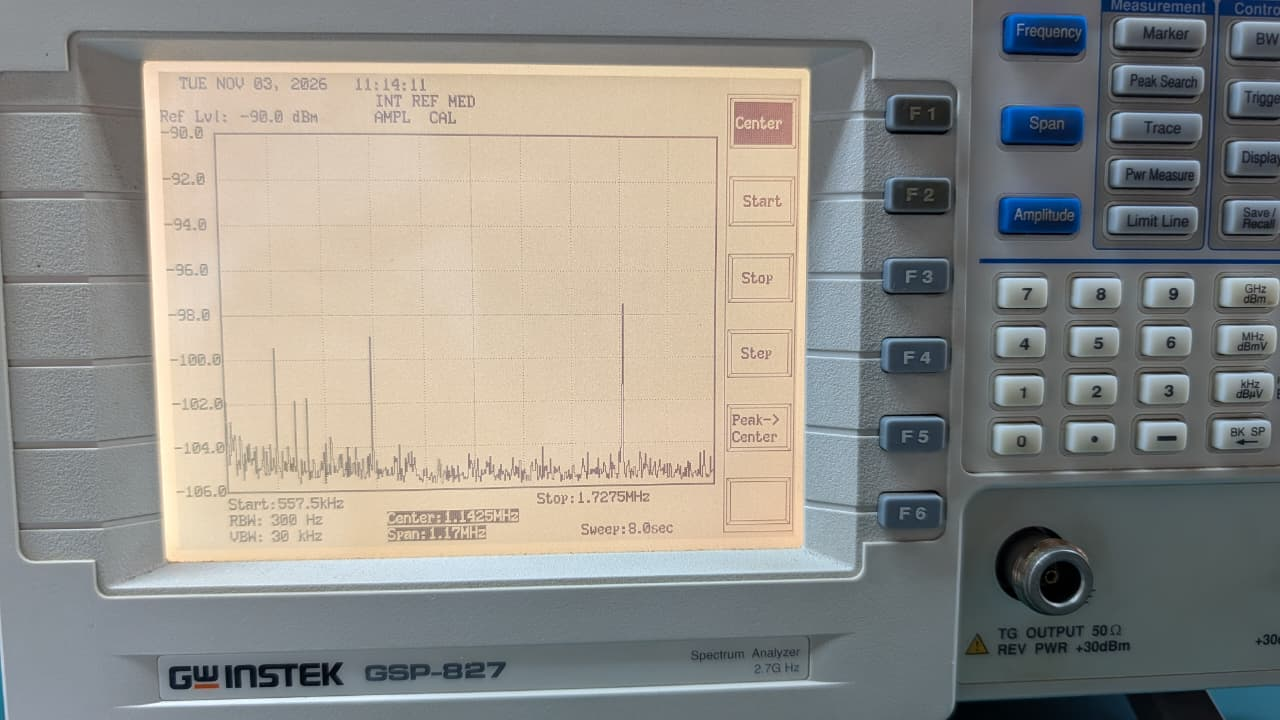
\includegraphics[width=0.85\textwidth]{am_completa.png}
    \caption{Exploración de la banda de radiodifusión en AM.}
    \label{fig:am_completa}
\end{figure}

\begin{figure}[H]
    \centering
    \begin{subfigure}[b]{0.49\textwidth}
        \centering
        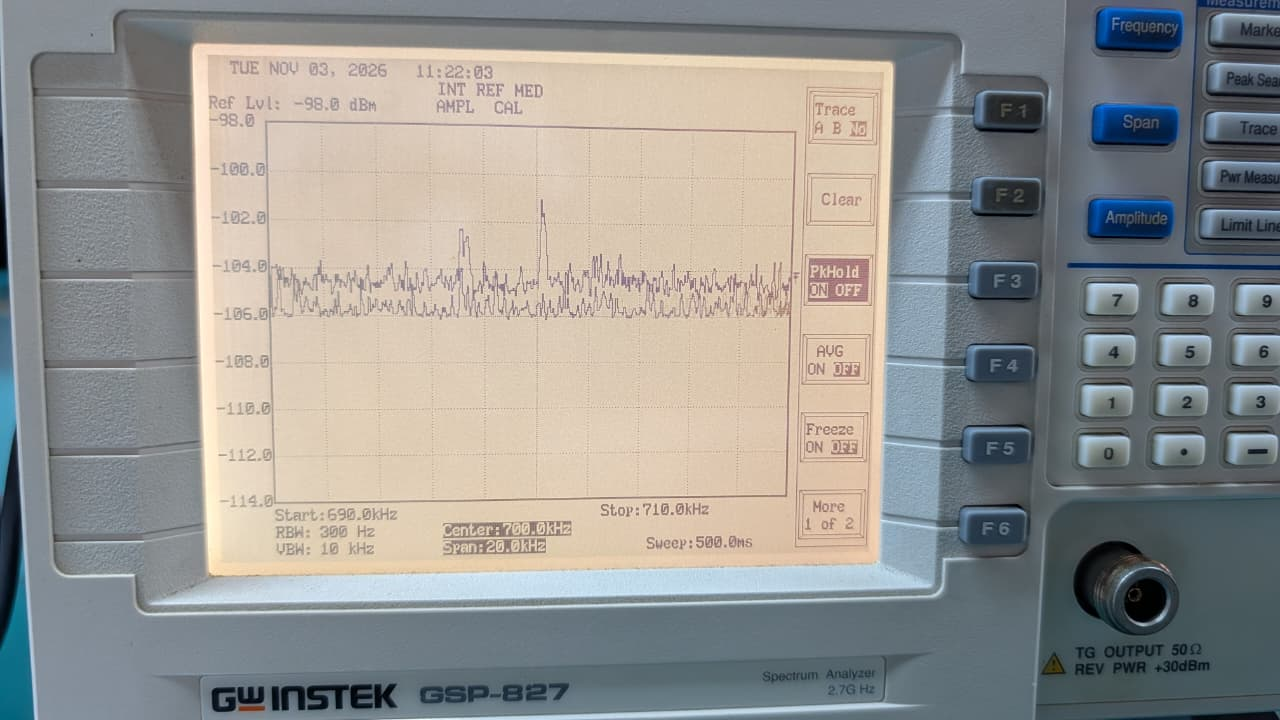
\includegraphics[width=\linewidth]{am_emisora1.png}
        \caption{Emisora 1 (Cadena 3, $700 \, [kHz]$).}
        \label{fig:am_emisora1}
    \end{subfigure}
    \hfill
    \begin{subfigure}[b]{0.49\textwidth}
        \centering
        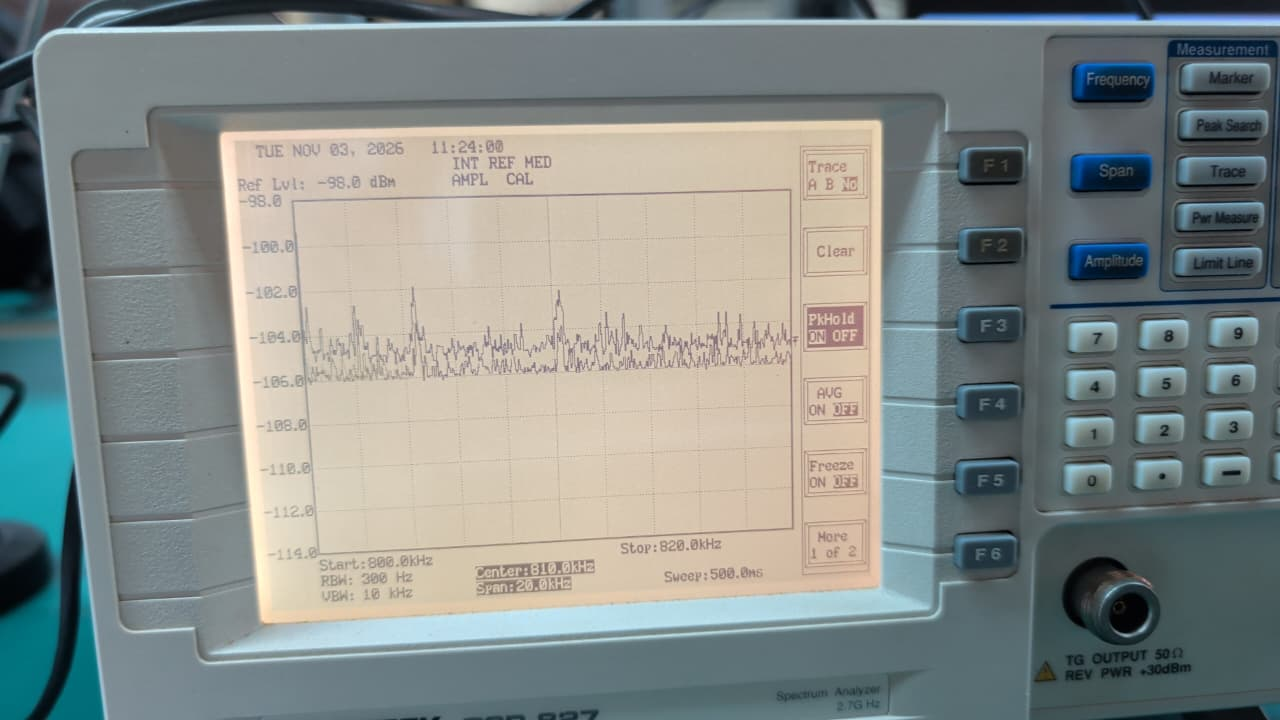
\includegraphics[width=\linewidth]{am_emisora2.png}
        \caption{Emisora 2 (Radio Mitre, $810 \, [kHz]$).}
        \label{fig:am_emisora2}
    \end{subfigure}
    \caption{Portadoras de las emisoras de AM observadas con un \textit{span} de $20 \, [kHz]$.}
    \label{fig:am_emisoras}
\end{figure}

\subsubsection*{Señal AM generada en el laboratorio}
Para observar el espectro de una AM con una modulante conocida, se conectó al analizador un generador de funciones GW Instek AFG-2125 con modulación interna (\autoref{fig:am_gen_parametros}).

\begin{table}[H]
    \centering
    \caption{Configuración del generador y del analizador para la señal AM generada.}
    \label{tab:am_generador}
    \begin{tabular}{p{8.5cm} p{5.8cm}}
        \toprule
        \textbf{Parámetro} & \textbf{Valor} \\
        \midrule
        \textbf{Generador (AFG-2125)} \\
        \midrule
        Portadora & $580 \, [kHz]$, $-20 \, [dBm]$ \\
        Modulante & $10 \, [kHz]$, senoidal y cuadrada (interna) \\
        Profundidad de modulación & $80 \, $\% ($m = 0{,}8$) \\
        \midrule
        \textbf{Analizador (GSP-827)} \\
        \midrule
        Frecuencia central / \textit{span} & $582 \, [kHz]$ / $1 \, [MHz]$ \\
        Nivel de referencia & $-20 \, [dBm]$ \\
        RBW / VBW & $9 \, [kHz]$ / $100 \, [kHz]$ \\
        Nivel de la portadora & $\approx -31 \, [dBm]$ \\
        Marcador en $674{,}5 \, [kHz]$ (senoidal / cuadrada) & $-73{,}7 \, [dBm]$ / $-56{,}1 \, [dBm]$ \\
        \bottomrule
    \end{tabular}
\end{table}

\begin{figure}[H]
    \centering
    \begin{subfigure}[b]{0.49\textwidth}
        \centering
        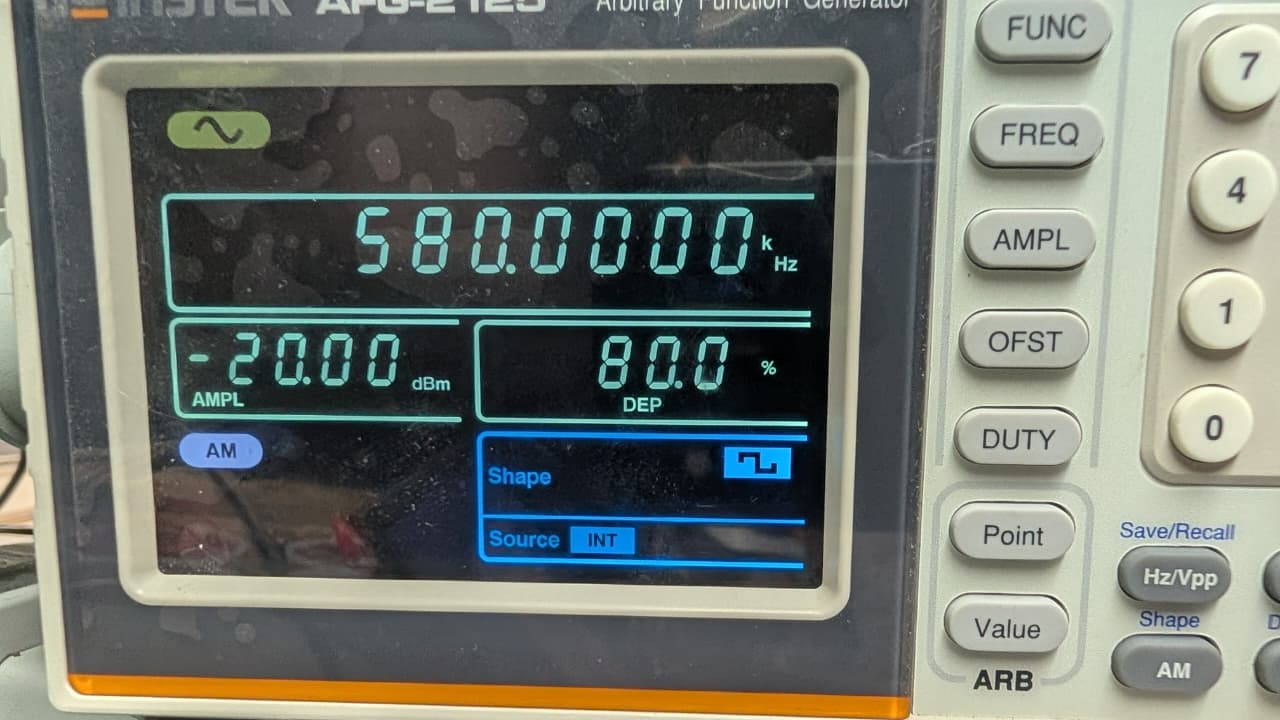
\includegraphics[width=\linewidth]{am_gen_portadora.png}
        \caption{Portadora.}
    \end{subfigure}
    \hfill
    \begin{subfigure}[b]{0.49\textwidth}
        \centering
        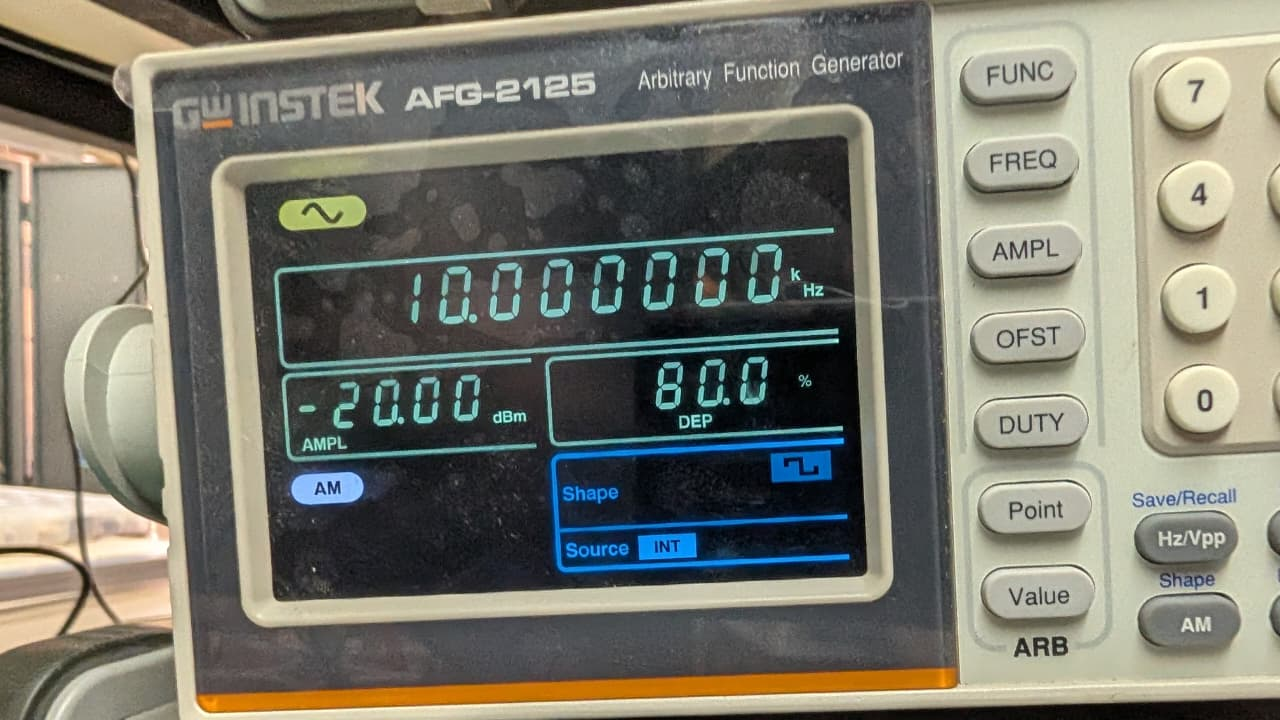
\includegraphics[width=\linewidth]{am_gen_modulante.png}
        \caption{Modulante.}
    \end{subfigure}
    \caption{Configuración del generador AFG-2125.}
    \label{fig:am_gen_parametros}
\end{figure}

\begin{figure}[H]
    \centering
    \begin{subfigure}[b]{0.49\textwidth}
        \centering
        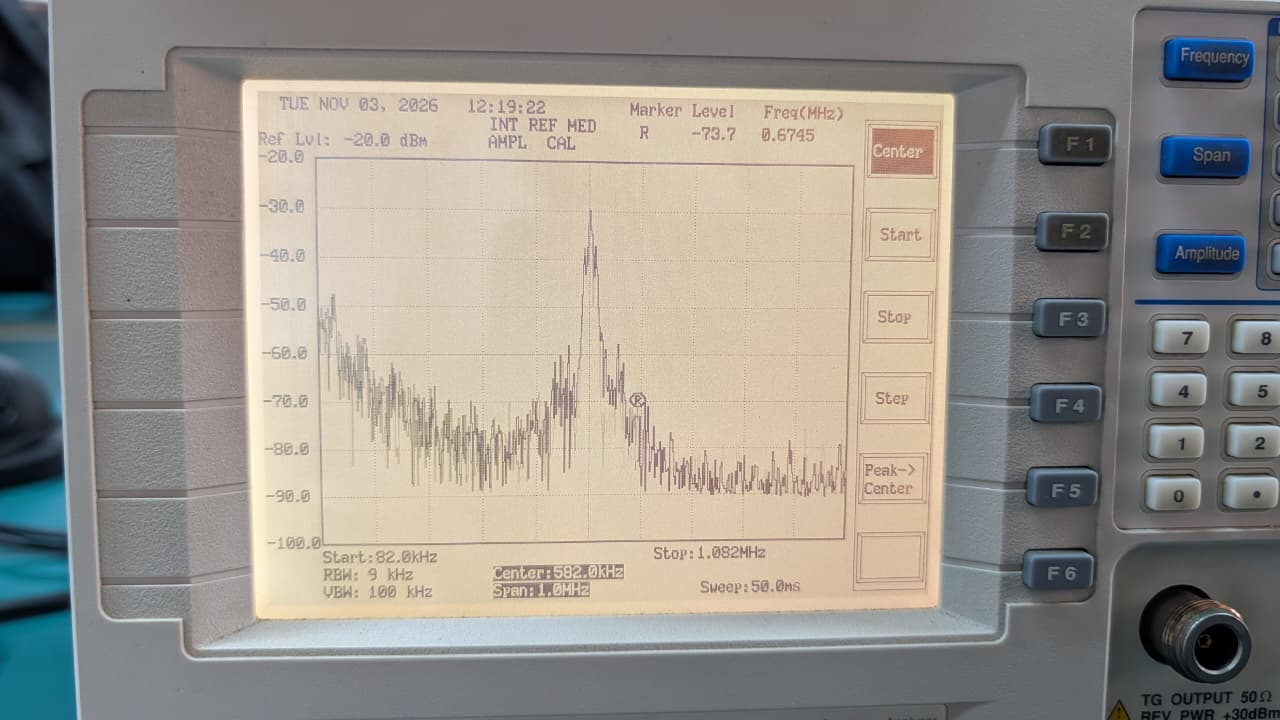
\includegraphics[width=\linewidth]{am_gen_seno.png}
        \caption{Modulante senoidal.}
        \label{fig:am_gen_seno}
    \end{subfigure}
    \hfill
    \begin{subfigure}[b]{0.49\textwidth}
        \centering
        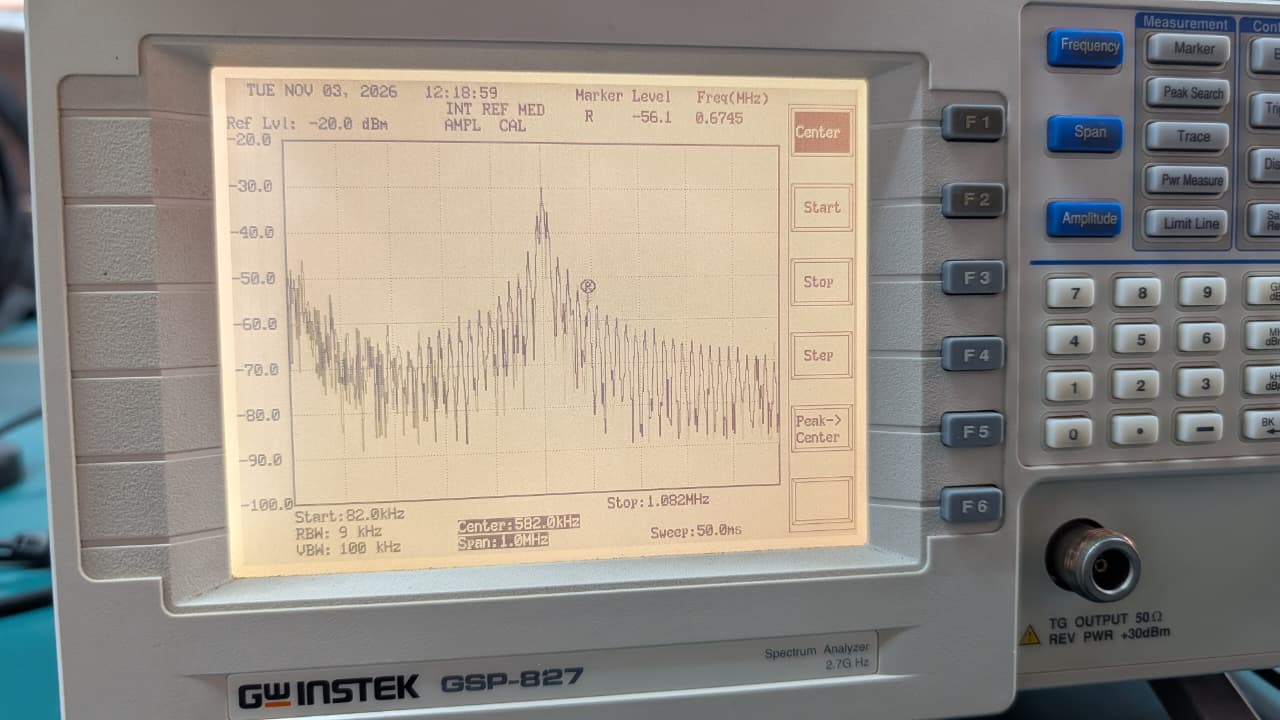
\includegraphics[width=\linewidth]{am_gen_cuadrada.png}
        \caption{Modulante cuadrada.}
        \label{fig:am_gen_cuadrada}
    \end{subfigure}
    \caption{Espectro de la señal AM generada ($f_c = 580 \, [kHz]$, $f_m = 10 \, [kHz]$, $m = 0{,}8$).}
    \label{fig:am_gen}
\end{figure}


\subsection{Análisis}

\subsubsection*{Componentes del espectro}
En las \autoref{fig:am_emisora1} y~\ref{fig:am_emisora2} se distingue la portadora en la frecuencia asignada a cada emisora, pero no las bandas laterales. La portadora se recibió con unos $-101$ a $-102 \, [dBm]$ pero las bandas laterales quedaron por debajo del piso de ruido y no pudieron observarse.

Se utilizó la retención de máximos (\textit{Peak Hold}), que conserva para cada frecuencia el mayor valor registrado en los barridos sucesivos. Esto permite acumular la envolvente de una emisión variable, pero también retiene los picos del ruido.

El bajo nivel recibido se atribuye a la antena utilizada (\autoref{fig:am_antena}): una antena interior de dos varillas en V, que es un dipolo pensado para los canales de VHF, donde cada varilla mide de un cuarto de longitud de onda. En la banda de AM, en cambio, $\lambda \approx 430 \, [m]$ en $700 \, [kHz]$, y con las varillas extendidas hasta un largo total de $1 \, [m]$ resulta $L / \lambda \approx 0{,}002$. A esto se suma la atenuación de la recepción en el interior del edificio.

\begin{figure}[H]
    \centering
    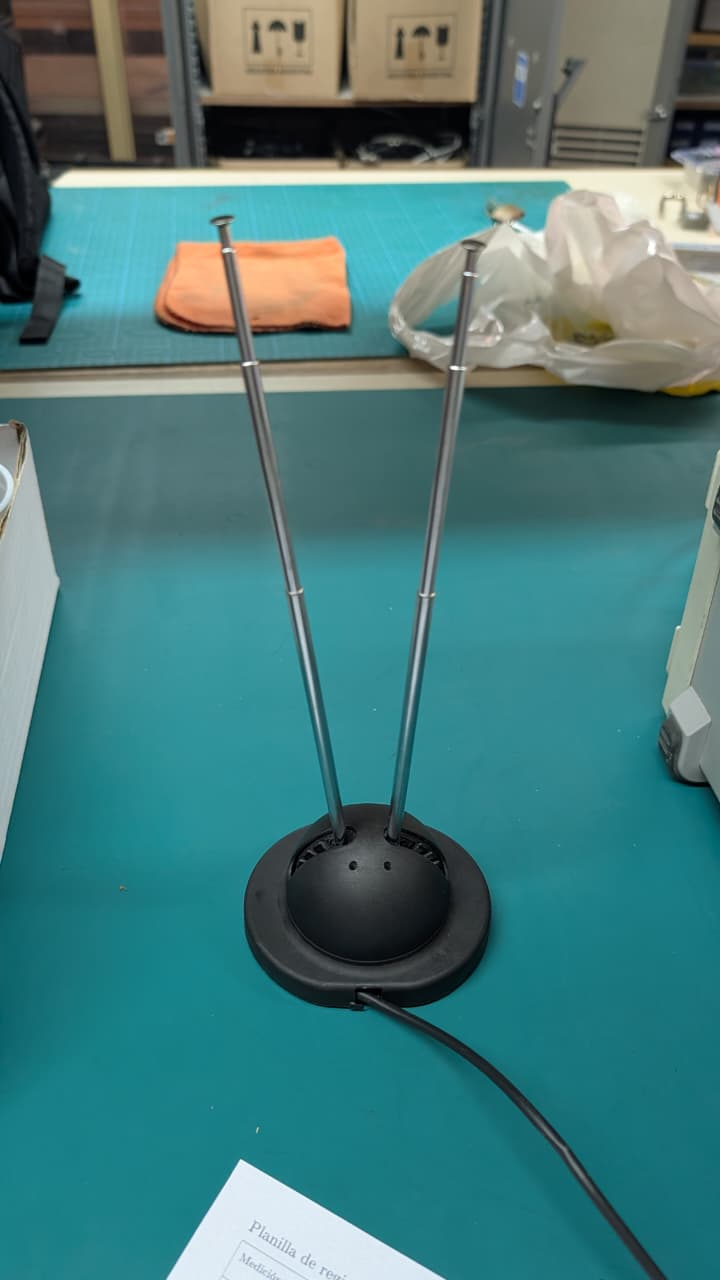
\includegraphics[width=0.25\textwidth]{am_antena.png}
    \caption{Antena interior de varillas telescópicas utilizada para la recepción en AM.}
    \label{fig:am_antena}
\end{figure}

\subsubsection*{Ancho de banda ocupado}
Para el ancho de banda se había previsto el criterio de ``$x$ dB'' de la Recomendación UIT-R SM.328, que lo mide entre las frecuencias donde el espectro cae $26 \, [dB]$ por debajo del máximo \cite{itu_sm328, itu_sm443}. Aplicarlo requiere que la portadora supere el piso de ruido en al menos $26 \, [dB]$, y en esta medición la diferencia fue de unos $3 \, [dB]$. Por eso el ancho de banda ocupado no pudo medirse. Según la canalización del CABFRA, con una separación de $10 \, [kHz]$ entre canales, se espera que la emisión ocupe como máximo unos $10 \, [kHz]$ \cite{cabfra}.

\subsubsection*{Canales adyacentes}
En las capturas con \textit{span} de $20 \, [kHz]$, los bordes de la pantalla coinciden con los canales adyacentes a $\pm 10 \, [kHz]$ de cada portadora, y en ninguno de ellos se observó una portadora. En el barrido de toda la banda (\autoref{fig:am_completa}) tampoco aparecen portadoras a $\pm 20 \, [kHz]$: las demás emisoras visibles están separadas varias decenas de kHz. Esto es coherente con la planificación, que evita asignar canales adyacentes a emisoras de una misma zona para limitar la interferencia entre ellas.

Se tuvo como limitación al piso de ruido: una emisora adyacente que llegue con menos de unos $-104 \, [dBm]$ no puede distinguirse, de modo que la ausencia de portadoras sólo indica que no hay señales por encima de ese nivel con la antena utilizada.

\subsubsection*{Máxima frecuencia modulante}
Con la separación de $10 \, [kHz]$ entre canales del CABFRA \cite{cabfra}, una emisión de doble banda lateral que no invada los canales adyacentes debe limitarse a unos $5 \, [kHz]$. Para verificarlo experimentalmente, la portadora debería superar el piso de ruido en varias decenas de dB, y el ancho debería medirse en retención de máximos durante el tiempo suficiente para que aparezcan las frecuencias altas del programa.

\subsubsection*{Señal AM generada: modulante senoidal y cuadrada}
Con una modulante senoidal, la \autoref{eq:am} predice una portadora y dos bandas laterales en $f_c \pm f_m = 570$ y $590 \, [kHz]$, con un nivel de $20 \log \frac{0{,}8}{2} \approx -8 \, [dBc]$ y un ancho de banda de $2 f_m = 20 \, [kHz]$. 

En la \autoref{fig:am_gen_seno}, sin embargo, se observa un único pico: las bandas laterales están a $10 \, [kHz]$ de la portadora, separación comparable al RBW de $9 \, [kHz]$, y con un \textit{span} de $1 \, [MHz]$. 

Se asume que hubo una configuración incorrecta del analizador, ya que no pudieron observarse las bandas laterales, por lo que el índice de modulación no pudo verificarse.

Con una modulante cuadrada, la envolvente alterna entre $1 + m$ y $1 - m$. Su serie de Fourier contiene sólo armónicas impares, de amplitud $\frac{4}{n \pi}$, de modo que cada una produce un par de bandas laterales en $f_c \pm n f_m$ con un nivel de
\begin{equation}
    N_{BL,n} - N_c = 20 \log \left( \frac{m}{2} \cdot \frac{4}{n \pi} \right), \qquad n = 1, 3, 5, \dots
    \label{eq:am_cuadrada}
\end{equation}

\begin{table}[H]
    \centering
    \caption{Nivel teórico de las bandas laterales con modulante cuadrada ($m = 0{,}8$, $f_m = 10 \, [kHz]$).}
    \label{tab:am_cuadrada}
    \begin{tabular}{c c c}
        \toprule
        \textbf{Armónica $n$} & \textbf{Frecuencias $[kHz]$} & \textbf{Nivel $[dBc]$} \\
        \midrule
        1 & $570$ y $590$ & $-5{,}9$ \\
        3 & $550$ y $610$ & $-15{,}4$ \\
        5 & $530$ y $630$ & $-19{,}8$ \\
        7 & $510$ y $650$ & $-22{,}8$ \\
        9 & $490$ y $670$ & $-24{,}9$ \\
        \bottomrule
    \end{tabular}
\end{table}

El espectro de la \autoref{fig:am_gen_cuadrada} coincide con esta predicción: un peine de componentes separadas $2 f_m = 20 \, [kHz]$, cuyo nivel disminuye lentamente y que se extiende por todo el \textit{span}.

La comparación muestra el efecto del contenido armónico de la modulante sobre el ancho de banda. Una senoidal ocupa $2 f_m$, mientras que una cuadrada, por sus flancos abruptos, tiene en teoría un ancho de banda infinito: en la práctica, uno que se extiende hasta donde sus armónicas caen bajo el piso de ruido. Por eso en radiodifusión el audio se limita en banda antes de modular, de modo que la emisión no invada los canales adyacentes.

\subsubsection*{Índice de modulación en una emisión de programa}
Con un único tono sinusoidal, el índice de modulación se obtiene de la diferencia de nivel entre una banda lateral y la portadora, a partir de la \autoref{eq:am}:
\begin{equation}
    m = \frac{2 E_{BL}}{E_c} = 2 \cdot 10^{(N_{BL} - N_c)/20}
    \label{eq:indice_am}
\end{equation}
Con una emisión comercial la \autoref{eq:indice_am} no puede aplicarse, porque la modulante no es un tono: tiene muchas componentes de frecuencia y amplitud variables, que reparten la potencia de las bandas laterales en un espectro continuo. No hay una única línea de banda lateral para medir, y su nivel depende del RBW y del instante. Tampoco puede suponerse que una emisora comercial module con $m = 1$: los procesadores de audio limitan los picos por debajo de la sobremodulación, y el índice varía todo el tiempo con el programa.

\subsection{Síntesis}
La AM imprime la información en la amplitud de la portadora. En el espectro esto se traduce en una portadora fija y dos bandas laterales simétricas, cuyo ancho es el doble de la máxima frecuencia modulante y cuyo nivel depende del índice de modulación.

En las emisoras recibidas, con una antena poco adecuada para la banda, sólo la portadora superó el piso de ruido, mientras que las bandas laterales, de menor nivel y repartidas en varios kHz, quedaron ocultas. Las emisoras se identificaron por su frecuencia, pero el ancho de banda y la máxima frecuencia modulante quedaron limitados al análisis teórico.

Con la señal del generador, en cambio, la modulante cuadrada produjo el peine de bandas laterales en las armónicas impares que predice su serie de Fourier, lo que muestra que el ancho de banda de una AM depende del contenido espectral de la modulante y justifica la limitación del audio en radiodifusión. Con la modulante senoidal, la configuración del analizador no permitió resolver las bandas laterales, por lo que el índice de modulación no pudo verificarse experimentalmente.
\section{Radiodifusión en FM}
\label{sec:fm}

\subsection{Modulación FM}
En la modulación de frecuencia, la frecuencia instantánea de la portadora se desvía en proporción a la señal modulante. Para un tono de frecuencia $f_m$ que produce una desviación máxima $\Delta f$, el índice de modulación es $\beta = \Delta f / f_m$ y la señal se desarrolla en funciones de Bessel de primera especie ($J_n(\beta)$) \cite{haykin}:
\begin{equation}
    v_{FM} = E_c \cos\left[2\pi f_c t + \beta \sin(2\pi f_m t)\right]
    = E_c \sum_{n=-\infty}^{\infty} J_n(\beta) \cos\left[2\pi (f_c + n f_m) t\right]
    \label{eq:fm}
\end{equation}

El espectro tiene infinitas componentes separadas $f_m$ entre sí, con amplitud $E_c J_n(\beta)$. Cada coeficiente da la amplitud relativa de la componente en $f_c + n f_m$: $J_0(\beta)$ corresponde a la portadora y $J_n(\beta)$, con $n \neq 0$, al par de bandas laterales de orden $n$. Como $J_{-n}(\beta) = (-1)^n J_n(\beta)$, las bandas laterales de un mismo orden tienen igual amplitud, y difieren sólo en el signo cuando $n$ es impar. Además, se cumple
\begin{equation}
    J_0^2(\beta) + 2 \sum_{n=1}^{\infty} J_n^2(\beta) = 1
\end{equation}
lo que indica que la potencia total es constante: la modulación sólo la redistribuye entre la portadora y las bandas laterales \cite{haykin}.

El número de componentes significativas crece con $\beta$. Con $\beta \ll 1$ (FM de banda angosta) sólo son apreciables $J_0 \approx 1$ y $J_1 \approx \beta/2$, y el espectro se parece al de una AM, con un par de bandas laterales. A medida que $\beta$ aumenta, la potencia se reparte en más pares, del orden de $\beta + 1$, por lo que casi toda la potencia queda en el ancho de banda que da la regla de Carson:

\begin{equation}
    B_T \approx 2 \left(\Delta f + f_m\right)
    \label{eq:carson}
\end{equation}

En la radiodifusión en FM la desviación máxima es de $\pm 75 \, [kHz]$ \cite{itu_bs450}. La señal que modula la portadora no es directamente el audio, sino la señal múltiplex estéreo, que agrupa en banda base las componentes de la \autoref{tab:fm_multiplex} (\autoref{fig:fm_multiplex}). El esquema es compatible con los receptores monofónicos, que sólo aprovechan la parte de $30 \, [Hz]$ a $15 \, [kHz]$, mientras que un receptor estéreo recupera ambos canales como $L = M + S$ y $R = M - S$.

\begin{table}[H]
    \centering
    \caption{Componentes de la señal múltiplex estéreo \cite{itu_bs450, itu_bs643}.}
    \label{tab:fm_multiplex}
    \renewcommand{\arraystretch}{1.3}
    \begin{tabular}{l l >{\raggedright\arraybackslash}p{7.6cm}}
        \toprule
        \textbf{Frecuencia} & \textbf{Componente} & \textbf{Función} \\
        \midrule
        $30 \, [Hz]$ a $15 \, [kHz]$ & $M = (L+R)/2$ & Suma de ambos canales: es la señal que reproduce un receptor monofónico. \\
        $19 \, [kHz]$ & Tono piloto & Referencia con la que el receptor regenera la subportadora de $38 \, [kHz]$, su segunda armónica. \\
        $23$ a $53 \, [kHz]$ & $S = (L-R)/2$ & Diferencia entre canales, en doble banda lateral con la subportadora de $38 \, [kHz]$ suprimida. \\
        $57 \, [kHz]$ & RDS (opcional) & Datos de identificación de la emisora y del programa, a $1187{,}5 \, [bit/s]$, sobre una subportadora suprimida enganchada a la tercera armónica del piloto. \\
        \bottomrule
    \end{tabular}
\end{table}

Las componentes se reparten la desviación máxima. Según la Recomendación UIT-R BS.450, $M$ y $S$ pueden alcanzar cada una el $90 \, $\% de la desviación, pero en condiciones distintas: con $L = R$ toda la señal está en $M$, y con $L = -R$ toda está en $S$. El tono piloto ocupa entre el $8$ y el $10 \, $\%, y el conjunto de las subportadoras adicionales, entre $53$ y $76 \, [kHz]$, no puede superar el $10 \, $\% \cite{itu_bs450}. Para el RDS se recomienda una desviación nominal de $\pm 2 \, [kHz]$ \cite{itu_bs643}.

Con la regla de Carson, la señal monofónica ocupa $2(75 + 15) = 180 \, [kHz]$ y la estéreo $2(75 + 53) = 256 \, [kHz]$. Este último valor es mayor que la separación de $200 \, [kHz]$ entre canales, porque la regla es conservadora: la desviación pico sólo se alcanza en los momentos de mayor nivel del programa, y las componentes de mayor frecuencia de la múltiplex no usan toda la desviación.

\begin{figure}[H]
    \centering
    \begin{tikzpicture}[x=0.165cm, y=0.05cm, font=\small]
        % Ejes
        \draw[-{Stealth[length=2mm]}] (0,0) -- (80,0) node[right] {$f \, [kHz]$};
        \draw[-{Stealth[length=2mm]}] (0,0) -- (0,108) node[above] {\% de $\Delta f_{max}$};
        \foreach \x in {0,15,19,23,38,53,57,76}
            \draw (\x,0) -- (\x,-1.5) node[below=1pt, font=\scriptsize] {\x};
        \foreach \y in {10,90,100}
            \draw (0,\y) -- (-1,\y) node[left, font=\scriptsize] {\y};
        \draw[densely dotted, gray] (0,100) -- (78,100);
        % M = (L+R)/2
        \draw[thick, blue!70!black, fill=blue!10] (0.03,0) -- (0.03,90) -- (15,90) -- (15,0);
        \node[blue!70!black, align=center] at (7.5,55) {$(L+R)/2$};
        % Piloto
        \draw[very thick, red!75!black] (19,0) -- (19,10);
        \node[red!75!black, above] at (19,10) {Piloto};
        % S = (L-R)/2, DBL con portadora suprimida en 38 kHz
        \draw[thick, green!45!black, fill=green!10] (23,0) -- (23,90) -- (37.97,90) -- (37.97,0);
        \draw[thick, green!45!black, fill=green!10] (38.03,0) -- (38.03,90) -- (53,90) -- (53,0);
        \node[green!45!black, align=center] at (30.5,45) {BLI};
        \node[green!45!black, align=center] at (45.5,45) {BLS};
        \node[green!45!black, fill=green!10, inner sep=1pt] at (38,76) {$(L-R)/2$, DBL-PS};
        \draw[dashed, green!45!black] (38,0) -- (38,90);
        \node[green!45!black, font=\scriptsize, fill=white, inner sep=1pt] at (38,22) {38 kHz};
        % RDS
        \draw[thick, orange!80!black, fill=orange!15] (55,0) -- (55,4) -- (59,4) -- (59,0);
        \node[orange!80!black, above] at (57,4) {RDS};
        % Zona de subportadoras adicionales
        \draw[decorate, decoration={brace, amplitude=4pt, mirror}] (53,-9) -- (76,-9)
            node[midway, below=5pt, font=\scriptsize, align=center] {Subportadoras adicionales\\($53$ a $76 \, [kHz]$, $\leq 10 \, $\%)};
    \end{tikzpicture}
    \caption{Espectro de la señal múltiplex estéreo en banda base (esquema propio basado en \cite{itu_bs450, itu_bs643}). La altura de cada componente indica su amplitud máxima como porcentaje de la desviación máxima; $M$ y $S$ alcanzan el $90 \, $\% en condiciones distintas, por lo que no lo hacen al mismo tiempo.}
    \label{fig:fm_multiplex}
\end{figure}

\subsection{Mediciones}

\subsubsection*{Exploración de la banda}
Se exploró la banda de $88$ a $108 \, [MHz]$ con un RBW de $9 \, [kHz]$ (\autoref{fig:fm_completa}). Sobre un piso de ruido de unos $-96 \, [dBm]$ se distinguen alrededor de una docena de emisoras, con niveles entre unos $-90$ y $-65 \, [dBm]$. Con un \textit{span} de $20 \, [MHz]$ cada emisora aparece como una línea, porque su ancho, del orden de $200 \, [kHz]$, ocupa apenas un punto de la traza.

\begin{figure}[H]
    \centering
    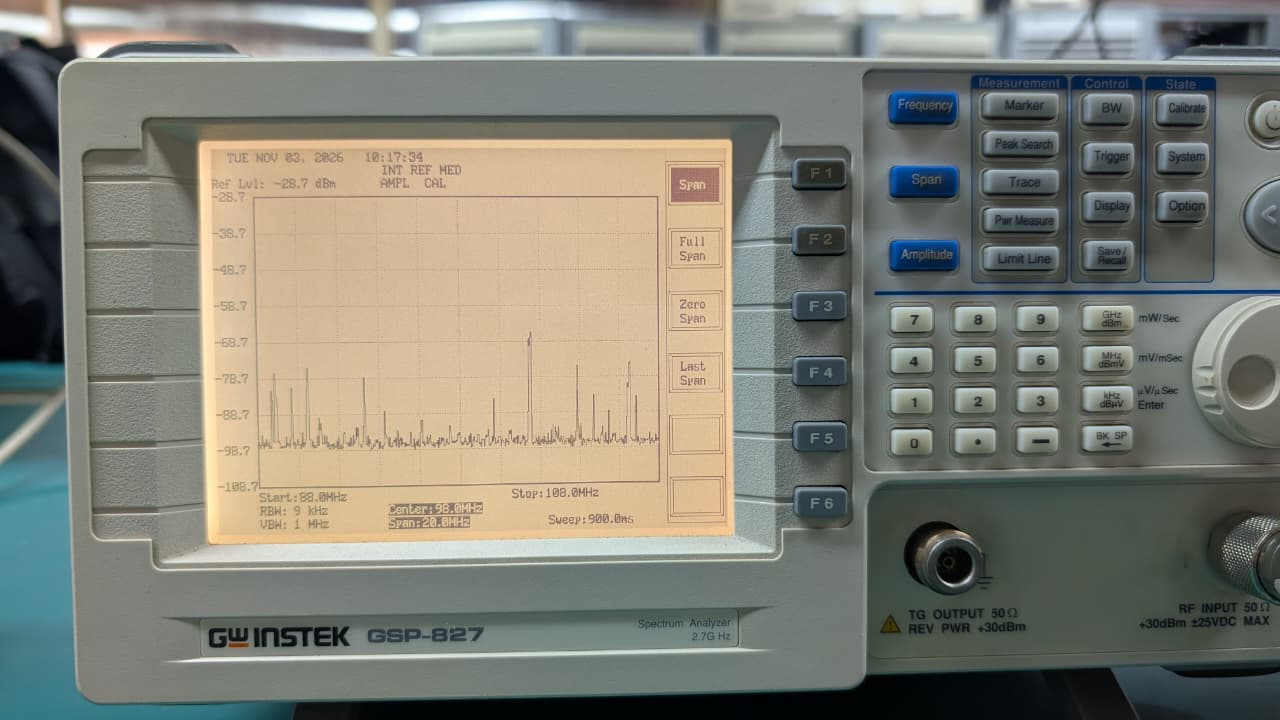
\includegraphics[width=0.8\textwidth]{fm_completa.png}
    \caption{Exploración de la banda de radiodifusión en FM.}
    \label{fig:fm_completa}
\end{figure}

\begin{table}[H]
    \centering
    \caption{Configuración del analizador y resultados en la banda de FM.}
    \label{tab:fm_resultados}
    \begin{tabular}{p{8.5cm} >{\raggedright\arraybackslash}p{5.8cm}}
        \toprule
        \textbf{Parámetro} & \textbf{Valor} \\
        \midrule
        Frecuencias de inicio y fin & $88$ a $108 \, [MHz]$ \\
        Frecuencia central & $98 \, [MHz]$ \\
        \textit{Span} & $20 \, [MHz]$ \\
        Nivel de referencia & $-28{,}7 \, [dBm]$ \\
        RBW / VBW & $9 \, [kHz]$ / $1 \, [MHz]$ \\
        \midrule
        \textbf{Emisora 1} \\
        \midrule
        Frecuencia de la portadora & $88{,}9 \, [MHz]$ \\
        Emisora identificada & No confirmada \\
        \textit{Span} & $600 \, [kHz]$ \\
        Nivel de referencia & $-60 \, [dBm]$ \\
        RBW / VBW & $3 \, [kHz]$ / $100 \, [kHz]$ \\
        Nivel de la portadora & $\approx -70 \, [dBm]$ (máximo de la envolvente) \\
        \midrule
        \textbf{Emisora 2} \\
        \midrule
        Frecuencia de la portadora & $102{,}3 \, [MHz]$ \\
        Emisora identificada & No confirmada \\
        \textit{Span} & $200 \, [kHz]$ \\
        Nivel de referencia & $-90 \, [dBm]$ \\
        RBW / VBW & $300 \, [Hz]$ / $30 \, [kHz]$ \\
        Nivel de la portadora & $\approx -92 \, [dBm]$ (componente máxima) \\
        \bottomrule
    \end{tabular}
\end{table}

\begin{figure}[H]
    \centering
    \begin{subfigure}[b]{0.485\textwidth}
        \centering
        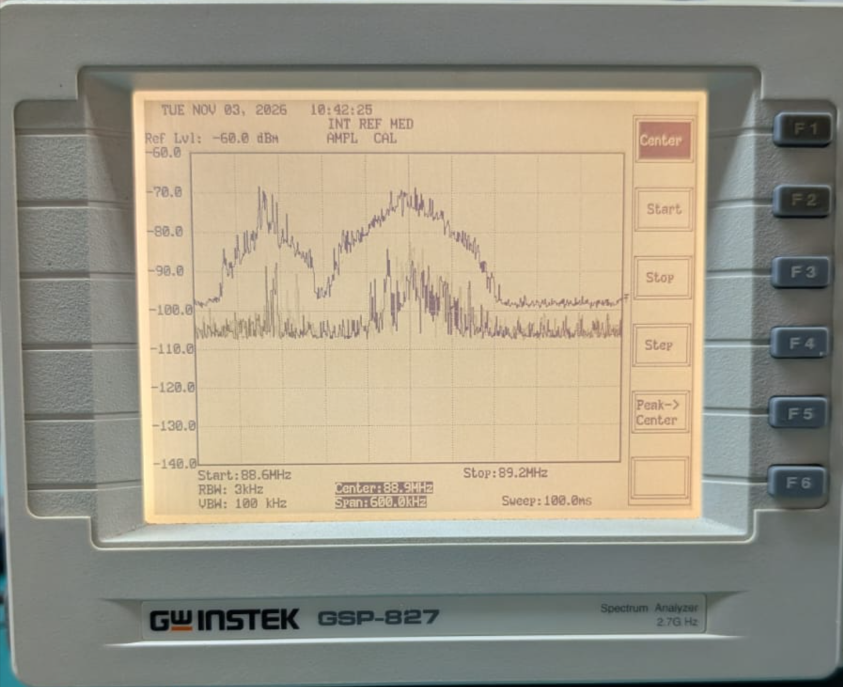
\includegraphics[width=\linewidth]{fm_emisora1.png}
        \caption{Emisora 1 ($88{,}9 \, [MHz]$).}
        \label{fig:fm_emisora1}
    \end{subfigure}
    \hfill
    \begin{subfigure}[b]{0.5\textwidth}
        \centering
        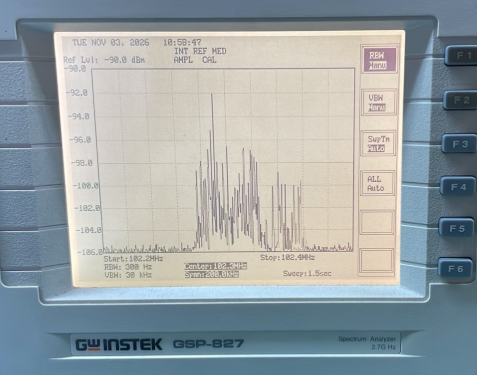
\includegraphics[width=\linewidth]{fm_emisora2.png}
        \caption{Emisora 2 ($102{,}3 \, [MHz]$).}
        \label{fig:fm_emisora2}
    \end{subfigure}
    \caption{Espectro de las emisoras de FM analizadas.}    \label{fig:fm_emisoras}
\end{figure}

Ninguna de las dos emisoras pudo confirmarse en el listado oficial de ENACOM. Según listados de emisoras no oficiales, la de $88{,}9 \, [MHz]$ correspondería a Pobre Johnny 88,9 FM y la de $102{,}3 \, [MHz]$ a CBA24 102,3 FM, ambas de la ciudad de Córdoba \cite{tuningaradio}.

\subsection{Análisis}

\subsubsection*{Ancho de banda ocupado}
Con una señal de programa, el espectro de FM no muestra una portadora fija y bandas laterales separadas, como con un tono: la energía se mueve dentro de un ``bloque'' de ancho variable alrededor de $f_c$. Por eso el ancho de banda se estimó sobre la envolvente en retención de máximos de la Emisora 1 (\autoref{fig:fm_emisora1}), entre los puntos que caen $26 \, [dB]$ por debajo del máximo \cite{itu_sm328}. Con el máximo en unos $-70 \, [dBm]$, ese nivel es de unos $-96 \, [dBm]$, y sobre la grilla se obtiene un ancho de banda de aproximadamente $220 \, [kHz]$. El resultado se compara con:
\begin{itemize}
    \item La separación entre canales de $200 \, [kHz]$ del CABFRA \cite{cabfra}: la emisión la supera levemente, de modo que sus flancos invaden los canales vecinos, aunque con un nivel muy inferior al del centro del canal.
    \item La regla de Carson, de $180 \, [kHz]$ para una emisión monofónica y de $256 \, [kHz]$ para una estéreo con la desviación máxima. El valor medido queda entre ambos, como se espera para una emisión estéreo que no alcanza la desviación máxima en forma permanente.
\end{itemize}

En la Emisora 2 no se estimó el ancho de banda. En un barrido simple con un RBW de $300 \, [Hz]$, el analizador observa cada frecuencia durante un instante muy breve. La \autoref{fig:fm_emisora2} muestra entonces un conjunto de líneas dispersas, que corresponden a las frecuencias donde había energía en el momento en que pasó el filtro, y que en ese barrido ocupan unos $100 \, [kHz]$. Además, las componentes superan el piso de ruido en sólo unos $13 \, [dB]$. Esta captura ilustra que el espectro de una FM con programa cambia en cada instante, y que para medir el ancho de banda ocupado es necesario acumular muchos barridos.

\subsubsection*{Canales adyacentes}
En la \autoref{fig:fm_emisora1} se observa una emisora en $88{,}7 \, [MHz]$, en el canal inmediatamente inferior al de la emisora analizada. Ambas llegan con niveles máximos similares, de unos $-70 \, [dBm]$, y sus envolventes se acercan hasta casi tocarse en la frecuencia intermedia, donde el nivel cae a unos $-98 \, [dBm]$, cerca del piso de ruido. La emisora de $88{,}7 \, [MHz]$ ocupa un bloque más angosto, de unos $150 \, [kHz]$, lo que podría deberse a una menor desviación o a una emisión monofónica. En el barrido de toda la banda (\autoref{fig:fm_completa}) las demás emisoras aparecen separadas por varios canales.

\subsubsection*{Índice de modulación y funciones de Bessel}
La componente de la frecuencia de la portadora tiene amplitud $E_c J_0(\beta)$ (\autoref{fig:fm_bessel}). Como $J_0$ se anula en $\beta = 2{,}405$, $5{,}520$, $8{,}654$, etc., con un tono conocido se puede subir la desviación hasta que la portadora desaparece del analizador y obtener $\Delta f = \beta f_m$ con gran precisión. Es el método de la portadora nula de Bessel, usado para calibrar moduladores de FM.

\begin{figure}[H]
    \centering
    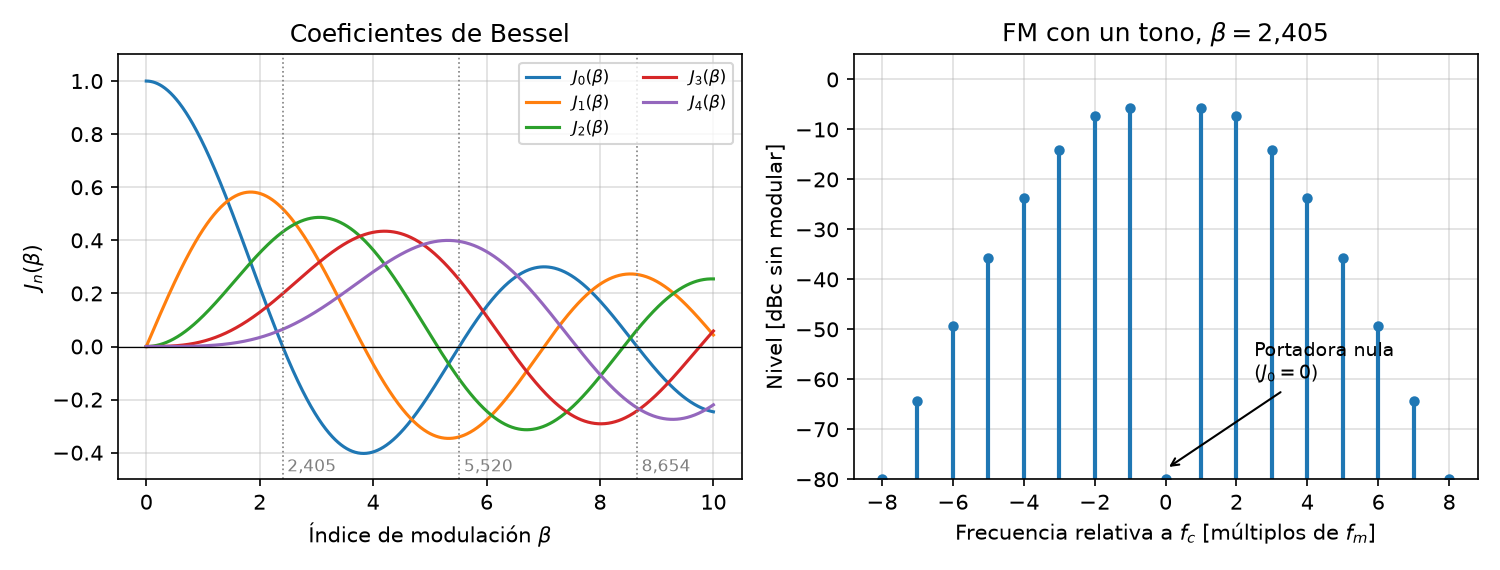
\includegraphics[width=\textwidth]{teoria/fm_bessel.png}
    \caption{Coeficientes de Bessel en función de $\beta$ y espectro de FM con portadora nula.}
    \label{fig:fm_bessel}
\end{figure}

Esta relación no permite medir el índice de modulación de una emisión de programa habitual, por tres razones:
\begin{itemize}
    \item La señal modulante es compleja: tiene muchas componentes de frecuencia y amplitud variables. El índice $\beta = \Delta f / f_m$ solo está definido para un tono, y con varios tonos aparecen productos de intermodulación con coeficientes $J_n(\beta_1) J_k(\beta_2) \cdots$.
    \item El espectro cambia continuamente con el contenido del programa, de modo que la línea de la portadora sube y baja todo el tiempo.
    \item La señal estéreo incluye, además del audio, el tono piloto, las bandas laterales de $S$ alrededor de $38 \, [kHz]$ y, si existe, el RDS, que también modulan la portadora.
\end{itemize}

\subsection{Síntesis}
La FM transmite la información en la frecuencia instantánea de la portadora, con amplitud constante. Esto la hace robusta frente al ruido y a las variaciones de amplitud del canal, y permite usar amplificadores no lineales. A cambio, ocupa un ancho de banda mucho mayor que la AM: unos $200 \, [kHz]$ contra $10 \, [kHz]$. En el analizador se ve como un bloque de energía de ancho variable alrededor de la frecuencia del canal, con potencia total constante y una distribución que cambia con el programa.

En la medición, la emisora de $88{,}9 \, [MHz]$ ocupó unos $220 \, [kHz]$ de ancho de banda, entre los valores de Carson para una emisión monofónica y una estéreo, y una emisora en el canal adyacente mostró que los flancos de canales contiguos llegan a acercarse hasta el piso de ruido.
\section{Televisión analógica}
\label{sec:tv_analogica}

\pendiente{Si en el laboratorio se recibió o generó una señal analógica, completar las mediciones de esta sección; si no, dejar el desarrollo conceptual e indicar que no se dispuso de señal.}

En Argentina, la televisión analógica usa la norma PAL-N: 625 líneas, 50 campos por segundo y canales de $6 \, [MHz]$ \cite{itu_bt470}. El CABFRA asigna a la televisión los canales 2 a 13 en VHF y 14 a 51 en UHF \cite{cabfra} (\autoref{tab:canalizacion}).

\subsection{Componentes del canal}
La \autoref{fig:tv_pal_n} muestra un esquema propio del espectro de un canal PAL-N, construido a partir de los parámetros de la norma \cite{itu_bt470}. Las frecuencias se miden desde el borde inferior del canal:
\begin{itemize}
    \item \underline{Portadora de video:} en $1{,}25 \, [MHz]$. Está modulada en amplitud por la señal de luminancia, con modulación negativa: el blanco corresponde a la menor amplitud y los pulsos de sincronismo a la máxima. La banda lateral superior se transmite completa, hasta $4{,}2 \, [MHz]$ por encima de la portadora, y de la inferior solo queda un vestigio de $0{,}75 \, [MHz]$.
    \item \underline{Subportadora de color:} en $1{,}25 + 3{,}582 = 4{,}83 \, [MHz]$. Las dos señales de diferencia de color, $U$ y $V$, la modulan en cuadratura (QAM) con portadora suprimida, y la fase de $V$ se invierte en cada línea, de donde viene el nombre PAL (\textit{Phase Alternating Line}). Al receptor se le envía una ráfaga (\textit{burst}) de la subportadora en cada línea, como referencia de fase.
    \item \underline{Portadora de audio:} en $1{,}25 + 4{,}5 = 5{,}75 \, [MHz]$, modulada en frecuencia con una desviación de $\pm 25 \, [kHz]$. Queda $0{,}25 \, [MHz]$ por debajo del borde superior del canal.
\end{itemize}

\begin{figure}[H]
    \centering
    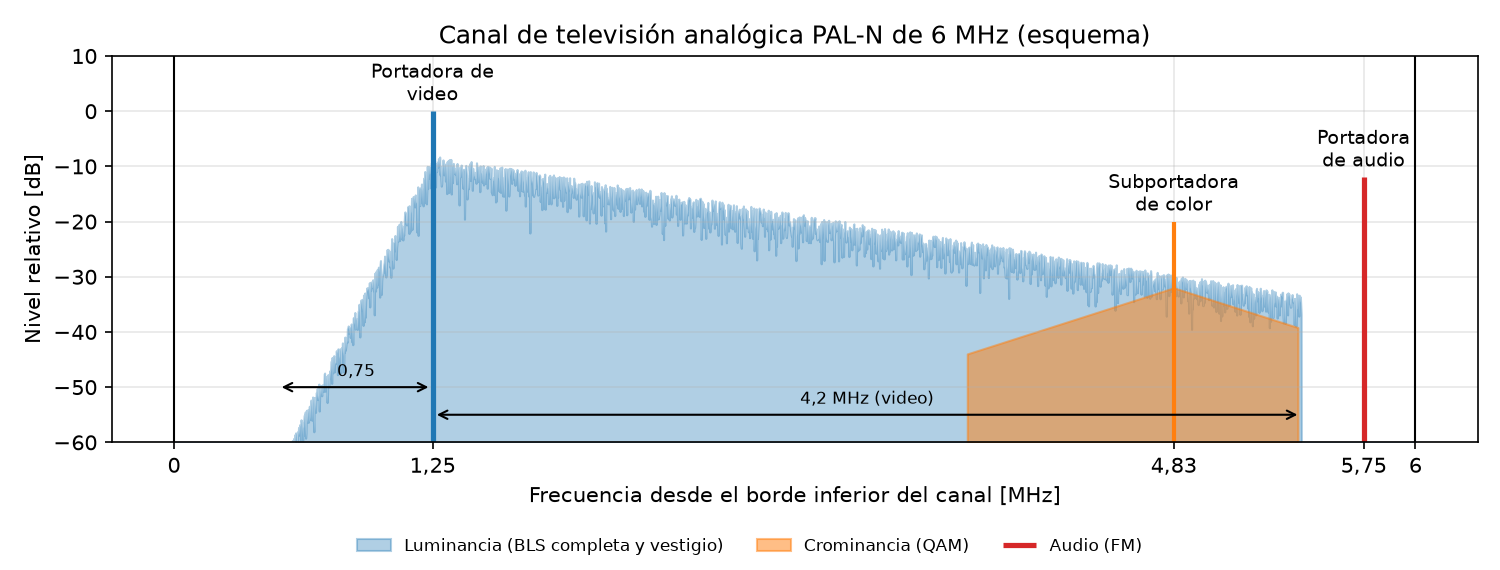
\includegraphics[width=\textwidth]{teoria/tv_pal_n.png}
    \caption{Espectro de un canal de televisión analógica PAL-N de $6 \, [MHz]$. Esquema propio a partir de la Rec. UIT-R BT.470 \cite{itu_bt470}.}
    \label{fig:tv_pal_n}
\end{figure}

\subsection{Mediciones}
\begin{table}[H]
    \centering
    \caption{Configuración del analizador y resultados para la señal de televisión analógica.}
    \label{tab:tv_resultados}
    \begin{tabular}{p{6.8cm} p{7.4cm}}
        \toprule
        \textbf{Parámetro} & \textbf{Valor} \\
        \midrule
        Canal y límites del canal & \pendiente{canal $N$, de $f_1$ a $f_2$ [MHz]} \\
        Frecuencia central / \textit{span} & \pendiente{} / \pendiente{$\approx 8 \, [MHz]$} \\
        Nivel de referencia / RBW / VBW & \pendiente{} \\
        Atenuación / preamplificación / unidad & \pendiente{} \\
        \midrule
        Portadora de video: frecuencia y nivel & \pendiente{} \\
        Subportadora de color: frecuencia y nivel & \pendiente{} \\
        Portadora de audio: frecuencia y nivel & \pendiente{} \\
        Relación audio/video & \pendiente{dB} \\
        Ancho de banda ocupado & \pendiente{MHz} \\
        \bottomrule
    \end{tabular}
\end{table}

\begin{figure}[H]
    \centering
    \pendiente{Captura del canal analógico (\texttt{Figuras/mediciones/tv\_analogica.png})}
    \caption{Espectro medido del canal de televisión analógica.}
    \label{fig:tv_medida}
\end{figure}

\subsection{Análisis}

\subsubsection*{Ancho de banda y banda lateral vestigial}
La señal ocupa unos $0{,}75 + 4{,}2 = 4{,}95 \, [MHz]$ de video, más el audio, dentro del canal de $6 \, [MHz]$. Con doble banda lateral, el video ocuparía $2 \times 4{,}2 = 8{,}4 \, [MHz]$ y no entraría en el canal. Con banda lateral única, en cambio, haría falta un filtro de corte abrupto justo en la portadora, imposible de construir sin distorsionar las bajas frecuencias del video, que son las de mayor energía (el nivel medio de la imagen y los sincronismos). La banda lateral vestigial es el compromiso entre ambas:
\begin{itemize}
    \item Se transmite la banda superior completa y un vestigio de la inferior, lo que permite un filtro de transmisión con una pendiente realizable.
    \item El receptor tiene un filtro de Nyquist, con una pendiente simétrica alrededor de la portadora: la suma de las dos bandas en la zona del vestigio reconstruye una respuesta plana.
    \item El receptor puede seguir usando un detector de envolvente.
\end{itemize}
\pendiente{Comparar con el ancho medido en la \autoref{fig:tv_medida}.}

\subsubsection*{Nivel del audio respecto del video}
La portadora de audio se transmite normalmente unos $10 \, [dB]$ por debajo del pico de la portadora de video. En la medición, el nivel de la portadora de video depende del contenido de la imagen, porque con modulación negativa una imagen clara reduce la amplitud media. Por eso la relación debe medirse con retención de máximos, para captar el nivel de los pulsos de sincronismo, que corresponden al pico de la envolvente, y con un RBW que contenga la portadora completa pero no las bandas laterales. \pendiente{Indicar la relación medida y las condiciones.}

\subsubsection*{Canales adyacentes}
\pendiente{Describir las señales detectadas en los canales vecinos.} El audio de un canal está a $0{,}25 \, [MHz]$ del borde superior y el vestigio del canal siguiente empieza $0{,}5 \, [MHz]$ por encima de ese borde, de modo que en una misma zona no se asignan canales adyacentes por aire. En las redes de cable, en cambio, se usan todos los canales contiguos, con niveles controlados.

\subsection{Síntesis}
En la televisión analógica PAL-N cada componente usa una modulación distinta dentro del mismo canal de $6 \, [MHz]$:
\begin{itemize}
    \item \underline{Video:} AM con banda lateral vestigial y modulación negativa.
    \item \underline{Color:} modulación en cuadratura de una subportadora en $3{,}58 \, [MHz]$, con alternancia de fase por línea, que ocupa la parte alta del espectro de luminancia sin interferirlo apreciablemente.
    \item \underline{Audio:} FM en una portadora $4{,}5 \, [MHz]$ por encima de la de video.
\end{itemize}

\section{Televisión digital terrestre (TDA)}
\label{sec:tda}

La Televisión Digital Abierta usa la norma ISDB-Tb \cite{decreto1148}, con canales de $6 \, [MHz]$ en la banda UHF, canales 14 a 51 \cite{cabfra}. El sistema se describe en detalle en la \autoref{sec:isdbtb}. Lo que importa para la medición es que la señal es OFDM: miles de subportadoras de igual nivel que ocupan $5{,}57 \, [MHz]$ del canal y que, en el analizador, forman una meseta plana con flancos abruptos (\autoref{fig:isdbtb_segmentos}).

\subsection{Mediciones}

\subsubsection*{Señales recibidas en el analizador}
Se exploró la banda de $470$ a $698 \, [MHz]$ con la antena de recepción y se registraron las señales de la \autoref{tab:tda_resultados}. La frecuencia central de cada canal se calculó con la \autoref{eq:canal_isdb}.

\begin{table}[H]
    \centering
    \caption{Señales de TDA observadas en el analizador y servicios decodificados por el receptor.}
    \label{tab:tda_resultados}
    \begin{tabular}{c c c c c p{4.6cm}}
        \toprule
        \textbf{Canal} & \textbf{$f_{central}$} & \textbf{Nivel} & \textbf{$B_{ocup}$} & \textbf{¿Decodifica?} & \textbf{Servicios} \\
        & \textbf{[MHz]} & \textbf{[dBm]} & \textbf{[MHz]} & & \\
        \midrule
        \pendiente{} & \pendiente{} & \pendiente{} & \pendiente{} & \pendiente{} & \pendiente{} \\
        \pendiente{} & \pendiente{} & \pendiente{} & \pendiente{} & \pendiente{} & \pendiente{} \\
        \pendiente{} & \pendiente{} & \pendiente{} & \pendiente{} & \pendiente{} & \pendiente{} \\
        \bottomrule
    \end{tabular}
\end{table}

\begin{table}[H]
    \centering
    \caption{Configuración del analizador para la TDA.}
    \label{tab:tda_config}
    \begin{tabular}{p{6.5cm} p{4cm} p{4cm}}
        \toprule
        \textbf{Parámetro} & \textbf{Exploración de banda} & \textbf{Detalle de un canal} \\
        \midrule
        Frecuencias de inicio y fin / central & $470$ a $698 \, [MHz]$ & \pendiente{} \\
        \textit{Span} & $228 \, [MHz]$ & \pendiente{$10 \, [MHz]$} \\
        Nivel de referencia & \pendiente{} & \pendiente{} \\
        RBW / VBW & \pendiente{} & \pendiente{$30$ a $100 \, [kHz]$} \\
        Atenuación / preamplificación / unidad & \pendiente{} & \pendiente{} \\
        \bottomrule
    \end{tabular}
\end{table}

\begin{figure}[H]
    \centering
    \pendiente{Captura de la banda UHF completa (\texttt{Figuras/mediciones/tda\_banda.png})}
    \caption{Exploración de la banda UHF de televisión digital.}
    \label{fig:tda_banda}
\end{figure}

\begin{figure}[H]
    \centering
    \pendiente{Captura de un canal ISDB-Tb en detalle (\texttt{Figuras/mediciones/tda\_canal.png})}
    \caption{Espectro de un canal ISDB-Tb.}
    \label{fig:tda_canal}
\end{figure}

\subsubsection*{Servicios decodificados por el receptor}
Se conectó la antena al televisor del laboratorio, se hizo una búsqueda automática de canales y se registraron los servicios recibidos (última columna de la \autoref{tab:tda_resultados}). \pendiente{Agregar fotografía de la lista de canales del televisor.}

\subsection{Análisis}

\subsubsection*{Ancho de banda ocupado}
En una señal OFDM, el ancho de banda ocupado se mide entre los flancos de la meseta: por ejemplo, donde el nivel cae $3 \, [dB]$ por debajo de la meseta, o como el ancho que contiene el $99 \,\text{\%}$ de la potencia \cite{itu_sm328}. El valor teórico es $5{,}57 \, [MHz]$ (13 segmentos de $428{,}57 \, [kHz]$), que deja unos $213 \, [kHz]$ de guarda a cada lado dentro del canal de $6 \, [MHz]$. \pendiente{Comparar con lo medido.}

Para medir el nivel de un canal digital no sirve la lectura de pico del analizador, porque la potencia está repartida en todo el ancho. El nivel del canal se obtiene integrando la densidad espectral:
\begin{equation}
    P_{canal} \, [dBm] = N_{meseta} \, [dBm] + 10 \log\left(\frac{5{,}57 \, [MHz]}{RBW}\right)
    \label{eq:potencia_canal}
\end{equation}
donde $N_{meseta}$ es el nivel leído sobre la meseta con un RBW dado. Muchos analizadores lo calculan directamente con la función de potencia de canal.

\subsubsection*{Forma del espectro y OFDM}
La meseta plana se explica porque las subportadoras tienen todas el mismo nivel medio y están tan juntas (de $1$ a $4 \, [kHz]$ de separación) que, con un RBW de decenas de kHz, el analizador no las resuelve y muestra su suma. Los flancos son abruptos porque el espectro de cada subportadora decae rápido fuera de la banda y porque el transmisor filtra la señal. En el centro de la meseta no aparece ninguna portadora destacada, porque no hay una portadora de referencia como en la televisión analógica. \pendiente{Señalar si se ven irregularidades en la meseta, que indicarían multitrayecto o ecos.}

\subsubsection*{Comparación con los servicios decodificados}
\pendiente{Comparar los canales vistos en el analizador con los que decodificó el receptor.} La presencia de una señal en el analizador no garantiza que se decodifique. El receptor necesita:
\begin{itemize}
    \item Un nivel por encima de su sensibilidad.
    \item Una relación señal a ruido mayor que la que pide la modulación de cada capa, que es mayor para 64-QAM que para QPSK.
    \item Que los ecos queden dentro del intervalo de guarda.
    \item Que no haya interferencias en el canal.
\end{itemize}
A la inversa, el receptor puede decodificar el segmento central (\textit{one-seg}, en QPSK) aunque no logre decodificar la capa HD, en 64-QAM.

\subsection{Síntesis}
La TDA argentina usa ISDB-Tb: OFDM en canales de $6 \, [MHz]$ divididos en 13 segmentos, que pueden agruparse en hasta tres capas jerárquicas con distinta modulación (DQPSK, QPSK, 16-QAM o 64-QAM) y distinta tasa de código. Así, un mismo canal transporta un servicio en alta definición para recepción fija y uno robusto para receptores móviles. El desarrollo completo está en la \autoref{sec:isdbtb}.

\newpage
\part*{Parte 2: Interpretación de niveles}
\addcontentsline{toc}{part}{Parte 2: Interpretación de niveles}
\section{Unidades utilizadas en las mediciones}
\label{sec:niveles}

\subsection{Decibeles absolutos y relativos}
\begin{itemize}
    \item \underline{dBm:} potencia relativa a $1 \, [mW]$, $P_{dBm} = 10 \log\left(P / 1 \, [mW]\right)$. Es una medida absoluta: $0 \, [dBm] = 1 \, [mW]$, $-30 \, [dBm] = 1 \, [\mu W]$ y $-60 \, [dBm] = 1 \, [nW]$.
    \item \underline{dB$\mu$V:} tensión relativa a $1 \, [\mu V]$. Como es un cociente de tensiones, se calcula como $V_{dB\mu V} = 20 \log\left(V / 1 \, [\mu V]\right)$. Es la unidad habitual en recepción de radiodifusión y en redes de cable, donde los niveles se especifican en tensión sobre $75 \, [\Omega]$.
    \item \underline{dBc:} nivel de una componente relativo al de la portadora, $N_{dBc} = N_{comp} - N_{portadora}$. Es una medida relativa: no depende de la impedancia ni de la ganancia del sistema, y por eso se usa para expresar bandas laterales, espurias, armónicos o ruido de fase.
\end{itemize}

\subsection{Relación entre potencia y tensión}
Sobre una resistencia $R$, una tensión eficaz $V$ disipa una potencia
\begin{equation}
    P = \frac{V^2}{R} \quad \Rightarrow \quad V = \sqrt{P R}
    \label{eq:p_v}
\end{equation}
Expresando $P$ en mW y $V$ en µV:
\begin{equation}
    V_{dB\mu V} = 20 \log\frac{\sqrt{P R}}{10^{-6}}
    = 10 \log\frac{P}{10^{-3}} + 10 \log\frac{10^{-3} R}{10^{-12}}
    = P_{dBm} + 90 + 10 \log R
    \label{eq:dbm_dbuv}
\end{equation}

Para los dos valores de impedancia habituales:
\begin{align}
    R = 50 \, [\Omega]: & \quad V_{dB\mu V} = P_{dBm} + 107{,}0 \\
    R = 75 \, [\Omega]: & \quad V_{dB\mu V} = P_{dBm} + 108{,}8
\end{align}
Por ejemplo, $-20 \, [dBm]$ equivalen a $87{,}0 \, [dB\mu V]$ ($22{,}36 \, [mV]$) sobre $50 \, [\Omega]$ y a $88{,}8 \, [dB\mu V]$ ($27{,}39 \, [mV]$) sobre $75 \, [\Omega]$. La diferencia entre ambos sistemas es $10 \log(75/50) = 1{,}76 \, [dB]$.

La \autoref{tab:conversion} resume algunas equivalencias.

\begin{table}[H]
    \centering
    \caption{Equivalencias entre dBm, potencia, tensión y dBµV para $50$ y $75 \, [\Omega]$.}
    \label{tab:conversion}
    \begin{tabular}{c c c c c c}
        \toprule
        \multirow{2}{*}{\textbf{dBm}} & \multirow{2}{*}{\textbf{Potencia}} & \multicolumn{2}{c}{\textbf{$50 \, [\Omega]$}} & \multicolumn{2}{c}{\textbf{$75 \, [\Omega]$}} \\
        \cmidrule(lr){3-4} \cmidrule(lr){5-6}
        & & \textbf{Tensión} & \textbf{dBµV} & \textbf{Tensión} & \textbf{dBµV} \\
        \midrule
        $0$   & $1 \, [mW]$   & $224 \, [mV]$  & $107{,}0$ & $274 \, [mV]$  & $108{,}8$ \\
        $-20$ & $10 \, [\mu W]$ & $22{,}4 \, [mV]$ & $87{,}0$ & $27{,}4 \, [mV]$ & $88{,}8$ \\
        $-40$ & $100 \, [nW]$ & $2{,}24 \, [mV]$ & $67{,}0$ & $2{,}74 \, [mV]$ & $68{,}8$ \\
        $-60$ & $1 \, [nW]$   & $224 \, [\mu V]$ & $47{,}0$ & $274 \, [\mu V]$ & $48{,}8$ \\
        $-107$ & $20 \, [fW]$ & $1{,}00 \, [\mu V]$ & $0{,}0$ & $1{,}22 \, [\mu V]$ & $1{,}8$ \\
        \bottomrule
    \end{tabular}
\end{table}

\subsection{Por qué hay que especificar la impedancia}
Un nivel en dBm indica una potencia y un nivel en dBµV, una tensión. Pasar de uno a otro requiere la \autoref{eq:p_v}, en la que interviene la resistencia sobre la que se desarrolla la tensión: la misma tensión de $1 \, [mV]$ entrega $20 \, [nW]$ ($-47 \, [dBm]$) sobre $50 \, [\Omega]$ y $13{,}3 \, [nW]$ ($-48{,}8 \, [dBm]$) sobre $75 \, [\Omega]$. Sin la impedancia, la conversión es ambigua en $1{,}76 \, [dB]$ entre los dos sistemas habituales.

En la práctica esto aparece al medir con el analizador de espectro, que tiene una entrada de $50 \, [\Omega]$ y mide en dBm, una red de $75 \, [\Omega]$ cuyos niveles se especifican en dBµV. Se pueden presentar tres casos:
\begin{itemize}
    \item \underline{Con adaptador de mínima pérdida:} a la lectura se le suma la atenuación del adaptador (unos $5{,}7 \, [dB]$) y se convierte con la ecuación de $75 \, [\Omega]$.
    \item \underline{Conexión directa:} se comete el error de desadaptación de $0{,}18 \, [dB]$ (\autoref{sec:equipamiento}).
    \item \underline{Analizador configurado en $75 \, [\Omega]$:} algunos instrumentos permiten indicar una impedancia de referencia de $75 \, [\Omega]$ y hacen la conversión internamente, pero eso no cambia la impedancia real de su entrada.
\end{itemize}

\section{Ejercicio de aplicación: índice de modulación de una señal AM}
\label{sec:ejercicio_am}

\textbf{Enunciado:} una señal AM ingresa al analizador de espectro con un nivel de portadora de $-20 \, [dBm]$ y bandas laterales de $-60 \, [dBm]$. Se requiere el índice de modulación $m$.

\textbf{Resolución en tensión:} se convierte cada nivel a tensión sobre $50 \, [\Omega]$ con la \autoref{eq:p_v}.
\begin{align}
    \text{Portadora:} \quad & P_c = 10^{-20/10} \, [mW] = 10 \, [\mu W]
    & E_c &= \sqrt{10^{-5} \cdot 50} = 22{,}36 \, [mV] \\
    \text{Banda lateral:} \quad & P_{BL} = 10^{-60/10} \, [mW] = 1 \, [nW]
    & E_{BL} &= \sqrt{10^{-9} \cdot 50} = 0{,}2236 \, [mV]
\end{align}

De la \autoref{eq:am}, cada banda lateral tiene amplitud $E_{BL} = \frac{m}{2} E_c$, de modo que
\begin{equation}
    m = \frac{2 E_{BL}}{E_c} = \frac{2 \cdot 0{,}2236}{22{,}36} = 0{,}02 = 2 \,\text{\%}
\end{equation}

\textbf{Resolución en dBc:} la banda lateral está $-60 - (-20) = -40 \, [dBc]$ respecto de la portadora. Con la \autoref{eq:indice_am}:
\begin{equation}
    m = 2 \cdot 10^{-40/20} = 2 \cdot 0{,}01 = 0{,}02 = 2 \,\text{\%}
\end{equation}

\textbf{Observaciones:}
\begin{itemize}
    \item El resultado no depende de la impedancia. Sobre $75 \, [\Omega]$ las tensiones son $27{,}39$ y $0{,}2739 \, [mV]$, pero su cociente es el mismo, porque la impedancia se cancela. Por eso el cálculo en dBc es el más directo.
    \item Un índice del $2 \,\text{\%}$ es muy bajo: las bandas laterales llevan solo $2 \cdot (m/2)^2 = 0{,}02 \,\text{\%}$ de la potencia de la portadora. Para que el método funcione, las bandas laterales tienen que quedar por encima del piso de ruido del analizador. Con $-60 \, [dBm]$ y un RBW de $9 \, [kHz]$ el margen es amplio, pero para índices menores conviene reducir el RBW.
    \item El cálculo supone modulación con un único tono sinusoidal, que es lo que permite identificar una única línea de banda lateral (\autoref{sec:am}).
\end{itemize}

\subsection{Ajustes recomendados del analizador}
Para las mediciones de la Parte 1, la cátedra recomienda:
\begin{itemize}
    \item Conector de desacople de continua, obligatorio.
    \item Medir solo señales de recepción.
    \item Nivel de referencia de $-30 \, [dBm]$, ajustable según la señal.
    \item \textit{Span} y frecuencias de inicio y fin según la banda medida.
    \item Ganancia de $5$ a $10 \, [dB]$.
    \item RBW de $9 \, [kHz]$ y VBW de $100 \, [kHz]$.
\end{itemize}
El RBW de $9 \, [kHz]$ es adecuado para explorar las bandas y para la FM y la televisión, pero es comparable al canal de AM de $10 \, [kHz]$, por lo que para resolver las bandas laterales de una emisora de AM conviene bajarlo a $1 \, [kHz]$ o menos (\autoref{sec:am}). El VBW, mayor que el RBW, deja la traza sin promediar. Si se lo reduce, la traza se suaviza y se lee mejor el nivel medio de una señal ruidosa como la OFDM.

\newpage
\part*{Parte 3: Investigación y desarrollo conceptual}
\addcontentsline{toc}{part}{Parte 3: Investigación y desarrollo conceptual}
\section{DVB-C}
\label{sec:dvbc}

DVB-C (\textit{Digital Video Broadcasting -- Cable}) es la norma del consorcio DVB para la transmisión de televisión digital por redes de cable, publicada por ETSI como EN 300 429 \cite{etsi_dvbc} y recogida por la UIT como Anexo A de la Recomendación J.83 \cite{itu_j83}.

\subsection{Tipo de red}
Se usa en redes de televisión por cable coaxial y en las redes híbridas fibra-coaxial (HFC): la señal sale de la cabecera por fibra hasta un nodo óptico, que la convierte a RF y la distribuye por coaxial de $75 \, [\Omega]$, con amplificadores y derivadores, hasta el abonado. El canal coaxial es mucho más benigno que el terrestre: no hay multitrayecto severo, la relación señal a ruido es alta (más de $30 \, [dB]$) y los niveles están controlados. Por eso DVB-C puede usar una modulación de un solo portador de alto orden, sin los mecanismos de robustez de la televisión terrestre.

\subsection{Modulación y codificación}
\begin{itemize}
    \item \underline{Modulación:} QAM de portadora única, con 16, 32, 64, 128 o 256 estados. Los más usados son 64-QAM y 256-QAM. Los símbolos se filtran con un coseno elevado de factor de \textit{roll-off} $\alpha = 0{,}15$.
    \item \underline{Codificación de canal:} aleatorización para dispersar la energía, código Reed-Solomon RS(204,188), que corrige hasta 8 bytes erróneos por paquete, y un entrelazador convolucional de profundidad 12. A diferencia de la norma terrestre, no hay código convolucional interno, porque el canal no lo requiere.
    \item \underline{Canal:} DVB-C se diseñó para canales de $8 \, [MHz]$ en Europa, pero la velocidad de símbolo es configurable, así que se adapta a canales de $6 \, [MHz]$.
\end{itemize}

La tasa útil de un canal es
\begin{equation}
    R_b = R_s \cdot \log_2 M \cdot \frac{188}{204}, \qquad R_s = \frac{B_{canal}}{1 + \alpha}
    \label{eq:dvbc}
\end{equation}
En un canal de $6 \, [MHz]$, $R_s = 6/1{,}15 = 5{,}22 \, [Mbaud]$. Con 256-QAM se obtienen $5{,}22 \cdot 8 \cdot 0{,}922 = 38{,}5 \, [Mbps]$ y con 64-QAM, $28{,}8 \, [Mbps]$. Con compresión H.264, un canal analógico de $6 \, [MHz]$ convertido a digital transporta entre 8 y 12 programas de definición estándar o 3 a 4 de alta definición.

La segunda generación, DVB-C2 (EN 302 769) \cite{etsi_dvbc2}, reemplaza la portadora única por OFDM y la codificación por LDPC con BCH, y admite constelaciones de hasta 4096-QAM. Con ello mejora la eficiencia en alrededor de un $30 \,\text{\%}$, aunque su adopción fue limitada porque los operadores migraron en paralelo hacia IPTV y DOCSIS.

\subsection{Transporte de los servicios de televisión}
DVB-C transporta un flujo de transporte MPEG-2 (\textit{Transport Stream}, TS) por canal: paquetes de 188 bytes que multiplexan el video y el audio comprimidos de varios programas, junto con las tablas de información de servicio:
\begin{itemize}
    \item \underline{PSI:} las tablas PAT y PMT, que indican qué paquetes forman cada programa.
    \item \underline{SI:} las tablas NIT, SDT y EIT, con los datos de la red, los nombres de los servicios y la guía de programación.
\end{itemize}
En la cabecera, los programas recibidos por satélite, por fibra o generados localmente se codifican, se multiplexan en varios TS y se modulan en canales QAM contiguos. Los servicios pagos se cifran con un sistema de acceso condicional (\textit{DVB Common Scrambling}): el abonado necesita un decodificador o un módulo de acceso condicional con su tarjeta. El receptor sintoniza el canal QAM, demodula el TS y extrae el programa elegido.

\subsection{Aplicación en Argentina}
Los grandes cableoperadores argentinos digitalizaron sus redes HFC con canales QAM, que conviven con los canales analógicos en la misma red y se reciben con un decodificador. Por ejemplo, Cablevisión desplegó en 2017 para su servicio Flow el decodificador ARRIS DCX4220, de diseño híbrido, que recibe tanto los canales QAM de la red de cable como contenido por IP \cite{lightwave_flow}. Las fuentes encontradas mencionan la recepción QAM, pero no detallan la norma ni la configuración de cada operador, por lo que la elección de DVB-C (frente al Anexo B de J.83, la norma norteamericana) debería confirmarse con la documentación técnica de cada uno.

\section{DOCSIS}
\label{sec:docsis}

DOCSIS (\textit{Data Over Cable Service Interface Specification}) es la familia de especificaciones de CableLabs para transmitir datos bidireccionales sobre redes de cable HFC \cite{docsis31, docsis40}, adoptada también por la UIT \cite{itu_j222}.

\subsection{Función dentro de la red de cable}
Una red de cable distribuye televisión en un solo sentido. DOCSIS le agrega un canal de datos bidireccional: reserva canales de RF del espectro descendente para los datos hacia el abonado y una banda baja para el sentido ascendente. Así, la misma red que lleva la TV ofrece acceso a Internet, telefonía IP y video sobre IP, sin un cableado nuevo.

\subsection{Equipos principales}
\begin{itemize}
    \item \underline{CMTS} (\textit{Cable Modem Termination System}): en la cabecera. Modula los canales descendentes, recibe los ascendentes y administra el acceso al medio: asigna a cada módem los intervalos en que puede transmitir.
    \item \underline{Red HFC:} fibra desde la cabecera hasta los nodos ópticos y, desde allí, coaxial con amplificadores bidireccionales, derivadores (\textit{taps}) y la acometida al abonado.
    \item \underline{Cable módem} (CM): en la casa del abonado. Sintoniza los canales DOCSIS, entrega la conexión por Ethernet o Wi-Fi y transmite en el sentido ascendente.
\end{itemize}

\begin{figure}[H]
    \centering
    \resizebox{\textwidth}{!}{%
    \begin{tikzpicture}[node distance=1.1cm, every node/.style={font=\small},
        caja/.style={draw, rounded corners, minimum height=1cm, minimum width=2.2cm, align=center, fill=blue!6}]
        \node[caja, fill=orange!12] (inet) {Internet /\\red IP};
        \node[caja, right=of inet] (cmts) {CMTS};
        \node[caja, below=0.6cm of cmts] (video) {Cabecera de\\video (QAM)};
        \node[caja, right=1.3cm of cmts] (comb) {Combinador\\RF};
        \node[caja, right=1.3cm of comb] (tx) {Transmisor y\\receptor óptico};
        \node[caja, right=1.6cm of tx] (nodo) {Nodo\\óptico};
        \node[caja, right=1.3cm of nodo] (amp) {Amplificador\\y \textit{taps}};
        \node[caja, above right=0.2cm and 1.0cm of amp, fill=green!8] (cm) {Cable\\módem};
        \node[caja, below right=0.2cm and 1.0cm of amp, fill=green!8] (stb) {Decodificador\\o TV};
        \draw[{Stealth}-{Stealth}] (inet) -- (cmts);
        \draw[{Stealth}-{Stealth}] (cmts) -- (comb);
        \draw[-{Stealth}] (video) -| (comb);
        \draw[{Stealth}-{Stealth}] (comb) -- (tx);
        \draw[{Stealth}-{Stealth}, very thick, red!70!black] (tx) -- node[above]{fibra} (nodo);
        \draw[{Stealth}-{Stealth}, very thick] (nodo) -- node[above]{coaxial} (amp);
        \draw[{Stealth}-{Stealth}] (amp.east) -- (cm.west);
        \draw[-{Stealth}] (amp.east) -- (stb.west);
        \node[draw, dashed, fit=(cmts)(video)(comb)(tx), inner sep=6pt, label=above:{Cabecera}] {};
    \end{tikzpicture}}
    \caption{Arquitectura de una red HFC con DOCSIS y televisión digital por cable.}
    \label{fig:docsis}
\end{figure}

\subsection{Sentidos de transmisión}
\begin{itemize}
    \item \underline{Descendente} (de la cabecera al abonado): el CMTS difunde a todos los módems del nodo. En DOCSIS 3.0 se usan canales QAM de $6 \, [MHz]$, de unos $38 \, [Mbps]$ cada uno, iguales a los de video digital. DOCSIS 3.1 introduce bloques OFDM de hasta $192 \, [MHz]$ con constelaciones de hasta 4096-QAM y codificación LDPC, y alcanza unos $10 \, [Gbps]$.
    \item \underline{Ascendente} (del abonado a la cabecera): el medio es compartido, así que los módems transmiten por turnos, en intervalos que asigna el CMTS (TDMA).
\end{itemize}

La \autoref{tab:docsis} resume la evolución de la familia.

\begin{table}[H]
    \centering
    \caption{Evolución de las versiones de DOCSIS (capacidades máximas aproximadas).}
    \label{tab:docsis}
    \begin{tabular}{c c c c p{5.4cm}}
        \toprule
        \textbf{Versión} & \textbf{Año} & \textbf{Descendente} & \textbf{Ascendente} & \textbf{Novedad principal} \\
        \midrule
        1.0 & 1997 & $40 \, [Mbps]$ & $10 \, [Mbps]$ & Primer estándar de módem por cable \\
        1.1 & 1999 & $40 \, [Mbps]$ & $10 \, [Mbps]$ & Calidad de servicio, telefonía IP \\
        2.0 & 2001 & $40 \, [Mbps]$ & $30 \, [Mbps]$ & Ascendente con A-TDMA y S-CDMA \\
        3.0 & 2006 & $1 \, [Gbps]$ & $200 \, [Mbps]$ & Agregación de canales, IPv6 \\
        3.1 & 2013 & $10 \, [Gbps]$ & $1$ a $2 \, [Gbps]$ & OFDM / OFDMA, LDPC, 4096-QAM \\
        4.0 & 2017 & $10 \, [Gbps]$ & $6 \, [Gbps]$ & Hasta $1{,}8 \, [GHz]$, \textit{Full Duplex} \\
        \bottomrule
    \end{tabular}
\end{table}

\subsection{DOCSIS, acceso a Internet y video sobre IP}
DOCSIS es, ante todo, la tecnología de acceso a Internet de las redes de cable: el CMTS funciona como un router de acceso y cada módem recibe una dirección IP. Como transporta IP, también sirve para distribuir video:
\begin{itemize}
    \item \underline{IPTV gestionada y OTT:} el decodificador recibe los programas como flujos IP por el módem. Es lo que hacen los decodificadores híbridos como el usado por Flow \cite{lightwave_flow}, que combinan la recepción QAM de los canales lineales con contenido IP a pedido.
    \item \underline{Migración a todo IP:} a medida que los operadores retiran los canales analógicos y QAM de video, ese espectro pasa a DOCSIS, y toda la televisión se entrega por IP.
\end{itemize}

\section{Video RF Overlay en redes FTTH}
\label{sec:rf_overlay}

El RF Overlay distribuye televisión sobre una red FTTH superponiendo, en una longitud de onda propia, el mismo espectro de RF que circula por una red de cable: los canales de $6 \, [MHz]$ de $47$ a $1.000 \, [MHz]$. El espectro completo de la cabecera modula en intensidad un láser de $1.550 \, [nm]$, viaja por la misma fibra y los mismos divisores ópticos que los datos de la red PON, y en la casa del abonado un receptor óptico lo convierte de nuevo en la señal de RF original, que se entrega por coaxial al televisor.

Desde el punto de vista del televisor, el RF Overlay es indistinguible de una red de cable, y desde el punto de vista de la red, es un servicio de difusión pura, independiente del sistema PON de datos con el que comparte la fibra. La Recomendación G.983.3 definió una banda de mejora de $1.550$ a $1.560 \, [nm]$ para servicios de video \cite{itu_g9833}, que G.984.5 conservó para GPON \cite{itu_g9845}.

\subsection{Integración con los servicios de datos}
La red PON de datos y el RF Overlay comparten toda la red de distribución óptica (ODN), pero se separan por longitud de onda (multiplexación WDM):
\begin{itemize}
    \item \underline{En la cabecera}, un combinador WDM une la salida de video, en $1.550 \, [nm]$, con el puerto PON de la OLT, que transmite en $1.490 \, [nm]$ y recibe en $1.310 \, [nm]$.
    \item \underline{En la ODN}, la fibra troncal, los divisores ópticos y las acometidas transportan las tres longitudes de onda sin distinción: los divisores son pasivos y de banda ancha.
    \item \underline{En la casa del abonado}, un filtro WDM separa el $1.550 \, [nm]$ hacia el receptor de video y deja pasar $1.490/1.310 \, [nm]$ hacia la ONT de datos.
\end{itemize}
Los dos servicios son independientes: el video no consume capacidad de los puertos GPON, y una falla de la OLT no interrumpe la televisión ni viceversa. Lo único que comparten es la ODN, y con ella su atenuación.

\begin{figure}[H]
    \centering
    \begin{tikzpicture}[every node/.style={font=\small},
        caja/.style={draw, rounded corners, minimum height=1.15cm, minimum width=2.7cm, align=center, fill=blue!6},
        int/.style={draw, fill=white, align=center, minimum width=2.4cm, minimum height=0.8cm},
        opt/.style={very thick, red!70!black}, rf/.style={thick, blue!60!black}, dat/.style={thick, green!55!black}]
        % Fila 1: cabecera de video
        \node[caja, fill=orange!12] (fuentes) at (0, 0) {Satélite, fibra\\y señales locales};
        \node[caja] (cab) at (3.7, 0) {Cabecera RF\\(moduladores\\QAM o ISDB-Tb)};
        \node[caja] (txo) at (7.4, 0) {Transmisor óptico\\$1.550 \, nm$};
        \node[caja] (edfa) at (11.1, 0) {Amplificador\\óptico EDFA};
        % Fila 2: datos y combinación
        \node[caja, fill=orange!12] (red) at (0, -2.4) {Red IP /\\enlace mayorista};
        \node[caja] (olt) at (3.7, -2.4) {OLT GPON\\$1.490 / 1.310 \, nm$};
        \node[caja] (wdm) at (11.1, -2.4) {Combinador\\WDM};
        % Fila 3: ODN
        \node[caja] (spl) at (11.1, -4.8) {Divisores ópticos\\$1{:}4$ y $1{:}16$};
        % Fila 4: abonado
        \node[int] (rxv) at (11.1, -8.0) {Receptor de\\video $1.550$};
        \node[int] (ontd) at (11.1, -9.2) {ONT de datos};
        \node[font=\small\bfseries] (ontlab) at (11.1, -7.2) {ONT con CATV};
        \node[draw, rounded corners, fill=green!8, fit=(ontlab)(rxv)(ontd), inner sep=5pt] (ont) {};
        \node[font=\small\bfseries] at (11.1, -7.2) {ONT con CATV};
        \node[int] (rxv) at (11.1, -8.0) {Receptor de\\video $1.550$};
        \node[int] (ontd) at (11.1, -9.2) {ONT de datos};
        \node[caja, fill=yellow!12] (tv) at (6.4, -8.0) {Televisores\\(coaxial $75 \, \Omega$)};
        \node[caja, fill=yellow!12] (lan) at (6.4, -9.4) {Router, Wi-Fi\\y STB IPTV};
        % Conexiones
        \draw[-{Stealth}] (fuentes) -- (cab);
        \draw[-{Stealth}, rf] (cab) -- node[above, font=\scriptsize]{RF} (txo);
        \draw[-{Stealth}, opt] (txo) -- node[above, font=\scriptsize]{$1.550$} (edfa);
        \draw[-{Stealth}, opt] (edfa) -- (wdm);
        \draw[{Stealth}-{Stealth}, dat] (red) -- (olt);
        \draw[{Stealth}-{Stealth}, opt] (olt) -- node[above, font=\scriptsize]{$1.490 / 1.310$} (wdm);
        \draw[{Stealth}-{Stealth}, opt] (wdm) -- node[right, font=\scriptsize]{fibra troncal ($3 \, \lambda$)} (spl);
        \draw[{Stealth}-{Stealth}, opt] (spl) -- node[pos=0.4, right, font=\scriptsize]{acometida} (ont);
        \draw[-{Stealth}, rf] (rxv) -- node[above, font=\scriptsize]{RF} (tv);
        \draw[{Stealth}-{Stealth}, dat] (ontd.west) -- node[above, font=\scriptsize]{Ethernet} (lan.east |- ontd.west);
        % Agrupaciones
        \node[draw, dashed, fit=(cab)(edfa)(olt)(wdm), inner sep=8pt, label={[font=\small]above:Oficina central / cabecera}] {};
        \node[draw, dashed, fit=(spl), inner sep=8pt, label={[font=\small]left:ODN}] {};
        \node[draw, dashed, fit=(ont)(tv)(lan), inner sep=8pt, label={[font=\small]below:Domicilio del abonado}] {};
        % Leyenda
        \node[align=left, font=\scriptsize, anchor=west] at (-1.35, -6.0) {%
            \textcolor{red!70!black}{\rule[0.5ex]{0.6cm}{1.5pt}} fibra óptica\\[2pt]
            \textcolor{blue!60!black}{\rule[0.5ex]{0.6cm}{1pt}} RF (video)\\[2pt]
            \textcolor{green!55!black}{\rule[0.5ex]{0.6cm}{1pt}} datos (eléctrico)};
    \end{tikzpicture}
    \caption{Diagrama en bloques de una red FTTH con RF Overlay.}
    \label{fig:rf_overlay}
\end{figure}

\subsection{Equipos y componentes principales}
\begin{itemize}
    \item \underline{Cabecera de RF:} reúne los canales de televisión. Recibe señales satelitales y de fibra, las decodifica y las vuelve a modular en canales de $6 \, [MHz]$, en DVB-C, ISDB-Tb o PAL-N, y las combina en un único espectro de RF, igual al de una red de cable.
    \item \underline{Transmisor óptico de $1.550 \, [nm]$:} convierte ese espectro de RF en una modulación de intensidad del láser. Como lleva muchos canales a la vez, debe ser muy lineal, para que no aparezcan productos de intermodulación de segundo y tercer orden sobre otros canales.
    \item \underline{Amplificador óptico EDFA:} amplifica directamente la señal óptica de $1.550 \, [nm]$. Compensa la atenuación de la división: una ODN 1:64 atenúa unos $25 \, [dB]$. Los EDFA de video tienen muchas salidas, una por cada puerto PON.
    \item \underline{Combinador WDM:} acopla el video de $1.550 \, [nm]$ con el puerto PON en una sola fibra, con bajas pérdidas de inserción y buen aislamiento entre longitudes de onda.
    \item \underline{Red de distribución óptica:} la misma ODN de la red de datos, con la fibra troncal, los divisores y las acometidas.
    \item \underline{Receptor de video:} un fotodiodo con un amplificador de RF de bajo ruido convierte la potencia óptica en la señal de RF original.
\end{itemize}

\subsection{Longitudes de onda}
La \autoref{fig:longitudes} resume el plan de longitudes de onda habitual cuando el RF Overlay comparte la ODN con GPON y, eventualmente, con XGS-PON \cite{itu_g9845, itu_g98071}:
\begin{itemize}
    \item \underline{GPON:} $1.490 \, [nm]$ en bajada y $1.310 \, [nm]$ en subida.
    \item \underline{Video RF Overlay:} $1.550$ a $1.560 \, [nm]$, en un solo sentido.
    \item \underline{XGS-PON:} $1.577 \, [nm]$ en bajada y $1.270 \, [nm]$ en subida.
\end{itemize}

\begin{figure}[H]
    \centering
    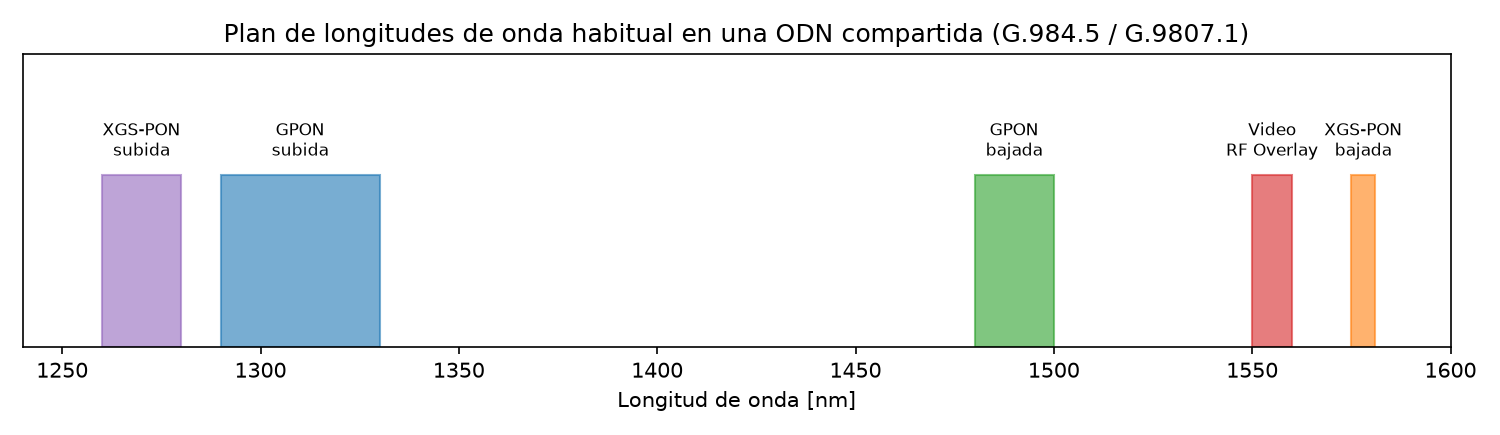
\includegraphics[width=\textwidth]{teoria/longitudes_onda.png}
    \caption{Longitudes de onda de GPON, XGS-PON y RF Overlay sobre una misma ODN.}
    \label{fig:longitudes}
\end{figure}

\subsection{Llegada de la señal al televisor}
El receptor óptico entrega por su salida coaxial el mismo espectro que sale de la cabecera. Desde allí, un cable coaxial de $75 \, [\Omega]$ (con divisores de RF si hay varios televisores) lleva la señal a cada aparato, como en una instalación de cable convencional. El televisor sintoniza los canales con su propio sintonizador: analógico PAL-N, ISDB-Tb, si la cabecera modula en esa norma, o DVB-C, si el televisor lo admite (y, si hace falta, un decodificador para canales cifrados).


\subsection{Diferencias entre RF Overlay e IPTV}
La \autoref{tab:overlay_iptv} compara ambas alternativas, con sus ventajas y limitaciones.

\begin{table}[H]
    \centering
    \small
    \caption{Comparación entre RF Overlay e IPTV en una red FTTH.}
    \label{tab:overlay_iptv}
    \renewcommand{\arraystretch}{1.2}
    \begin{tabular}{p{2.6cm} >{\raggedright\arraybackslash}p{5.9cm} >{\raggedright\arraybackslash}p{5.9cm}}
        \toprule
          & \textbf{RF Overlay} & \textbf{IPTV} \\
        \midrule
        \textbf{Transporte} & Espectro de RF completo, en modulación de intensidad a $1.550 \, [nm]$ & Paquetes IP multicast dentro del canal de datos de la PON \\
        \midrule
        \textbf{Distribución} & Difusión: los canales llegan siempre a todos los abonados & Bajo demanda: solo viajan los canales que se están mirando \\
        \midrule
        \textbf{Recepción} & Sintonizador del televisor, por coaxial & Decodificador IP (STB) o aplicación, por HDMI o Wi-Fi \\
        \midrule
        \textbf{Ventajas} &
        \begin{itemize}[nosep, leftmargin=*, before=\vspace{-0.6\baselineskip}, after=\vspace{-\baselineskip}]
            \item Los televisores existentes funcionan sin decodificador.
            \item Cada televisor de la casa sintoniza por su cuenta, sin equipos adicionales.
            \item No carga la red de datos, y el cambio de canal es tan rápido como el del sintonizador.
            \item Fácil migrar de una red HFC.
        \end{itemize} &
        \begin{itemize}[nosep, leftmargin=*, before=\vspace{-0.6\baselineskip}, after=\vspace{-\baselineskip}]
            \item Una sola red IP para todos los servicios, sin equipamiento óptico de video.
            \item Servicios interactivos: video a pedido, programación diferida y grabación en red.
            \item Cantidad de canales casi ilimitada, porque solo se transportan los que se miran.
        \end{itemize} \\
        \vspace{1pt}\\
        \midrule
        \textbf{Limitaciones} &
        \begin{itemize}[nosep, leftmargin=*, before=\vspace{-0.6\baselineskip}, after=\vspace{-\baselineskip}]
            \item Requiere equipamiento óptico de alta linealidad y potencia (transmisores, EDFA), costoso y específico para video.
            \item La CNR depende de la potencia óptica recibida, lo que exige un presupuesto óptico propio, más ajustado con canales analógicos que con digitales.
            \item Los canales pagos requieren acceso condicional en un decodificador.
        \end{itemize} &
        \begin{itemize}[nosep, leftmargin=*, before=\vspace{-0.6\baselineskip}, after=\vspace{-\baselineskip}]
            \item Necesita un STB o un televisor inteligente con aplicación por cada pantalla.
            \item Consume capacidad de los puertos PON y del enlace mayorista.
            \item Requiere una red con multicast, IGMP y calidad de servicio bien configurados.
            \item Es sensible a la congestión y a la pérdida de paquetes.
        \end{itemize} \\
        \vspace{1pt}\\
        \bottomrule
    \end{tabular}
\end{table}
\section{ISDB-Tb}
\label{sec:isdbtb}

ISDB-Tb (\textit{Integrated Services Digital Broadcasting -- Terrestrial, Brazilian version}) es la norma de televisión digital terrestre que Argentina adoptó en 2009 para la Televisión Digital Abierta \cite{decreto1148}. Toma la capa física de la norma japonesa ISDB-T (ARIB STD-B31) \cite{arib_b31}, recogida por la UIT en la Recomendación BT.1306 \cite{itu_bt1306}, con las modificaciones brasileñas de la norma ABNT NBR 15601 \cite{abnt15601}:
\begin{itemize}
    \item Compresión de video H.264 / MPEG-4 AVC, en lugar de MPEG-2.
    \item Audio AAC.
    \item Middleware de interactividad Ginga.
    \item Canales de $6 \, [MHz]$.
\end{itemize}

\subsection{Principio de funcionamiento de OFDM}
OFDM (\textit{Orthogonal Frequency Division Multiplexing}) divide el flujo de datos en miles de subflujos lentos, cada uno de los cuales modula una subportadora distinta. Las subportadoras están separadas exactamente $\Delta f = 1/T_u$, la inversa de la duración útil del símbolo. Con esa separación son ortogonales: en el centro del espectro de cada una, las demás pasan por cero (\autoref{fig:ofdm}), de modo que se solapan sin interferirse. La modulación y la demodulación se hacen con la transformada rápida de Fourier (IFFT en el transmisor, FFT en el receptor).

\begin{figure}[H]
    \centering
    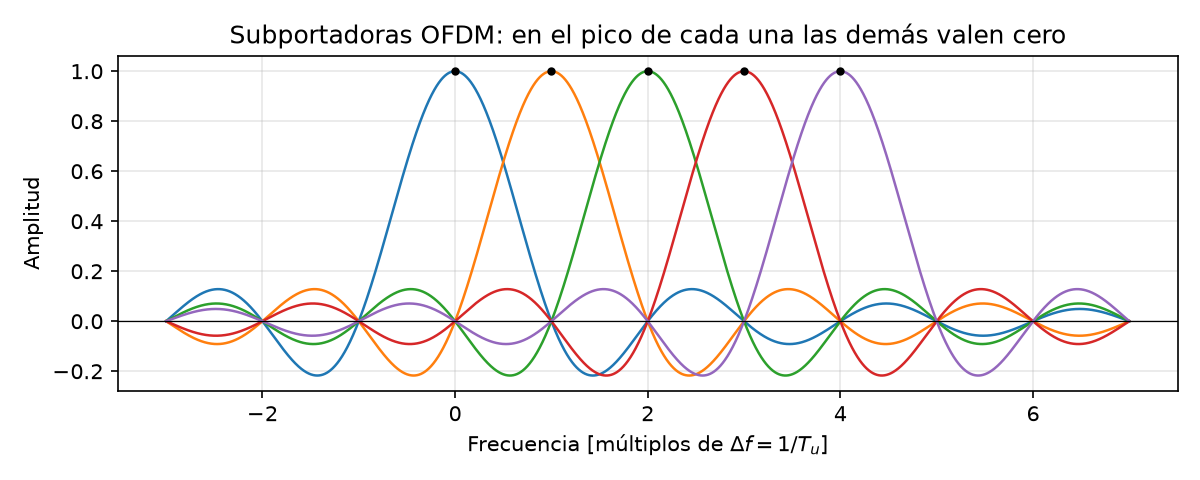
\includegraphics[width=0.8\textwidth]{teoria/ofdm_subportadoras.png}
    \caption{Espectros de las subportadoras OFDM: cada una tiene su máximo donde las demás se anulan (esquema propio).}
    \label{fig:ofdm}
\end{figure}

La ventaja frente a una portadora única es la robustez al multitrayecto. Cada símbolo OFDM dura cientos de microsegundos, mucho más que el retardo de los ecos. Además, a cada símbolo se le antepone un intervalo de guarda $T_g$, una copia de su parte final, de duración $1/4$, $1/8$, $1/16$ o $1/32$ de $T_u$. Si los ecos llegan dentro del intervalo de guarda no producen interferencia entre símbolos, y el efecto de cada eco sobre cada subportadora se reduce a un cambio de amplitud y de fase, que el receptor corrige con las portadoras piloto. Esto también permite las redes de frecuencia única (SFN), en las que varios transmisores emiten el mismo canal en la misma frecuencia.

ISDB-Tb tiene tres modos, que difieren en el tamaño de la FFT (\autoref{tab:modos}). Los modos con más subportadoras tienen símbolos más largos y toleran ecos más largos, pero son más sensibles al efecto Doppler en la recepción móvil.

\begin{table}[H]
    \centering
    \caption{Modos de transmisión de ISDB-Tb en canales de $6 \, [MHz]$ \cite{arib_b31, abnt15601}.}
    \label{tab:modos}
    \begin{tabular}{c c c c c c}
        \toprule
        \textbf{Modo} & \textbf{FFT} & \textbf{Subportadoras} & \textbf{Por segmento} & \textbf{$\Delta f$ [kHz]} & \textbf{$T_u$ [µs]} \\
        \midrule
        1 & 2k & 1.405 & 108 & $3{,}968$ & $252$ \\
        2 & 4k & 2.809 & 216 & $1{,}984$ & $504$ \\
        3 & 8k & 5.617 & 432 & $0{,}992$ & $1.008$ \\
        \bottomrule
    \end{tabular}
\end{table}

\subsection{Organización del canal en segmentos}
El ancho útil se divide en 13 segmentos OFDM de $6/14 \, [MHz] = 428{,}57 \, [kHz]$ cada uno, que en total ocupan $5{,}57 \, [MHz]$ del canal de $6 \, [MHz]$ (\autoref{fig:isdbtb_segmentos}). Cada segmento tiene subportadoras de datos, pilotos dispersos para estimar el canal y portadoras de control:
\begin{itemize}
    \item \underline{TMCC}: llevan la configuración de la transmisión (modulación, tasa de código y cantidad de segmentos de cada capa), de modo que el receptor se configura solo.
    \item \underline{AC}: llevan información auxiliar, como las alertas de emergencia EWBS.
\end{itemize}
Los segmentos se numeran del 0 al 12 desde el centro del canal hacia afuera. El segmento 0 ocupa el centro, lo que permite que un receptor de banda angosta decodifique solo ese segmento.

\begin{figure}[H]
    \centering
    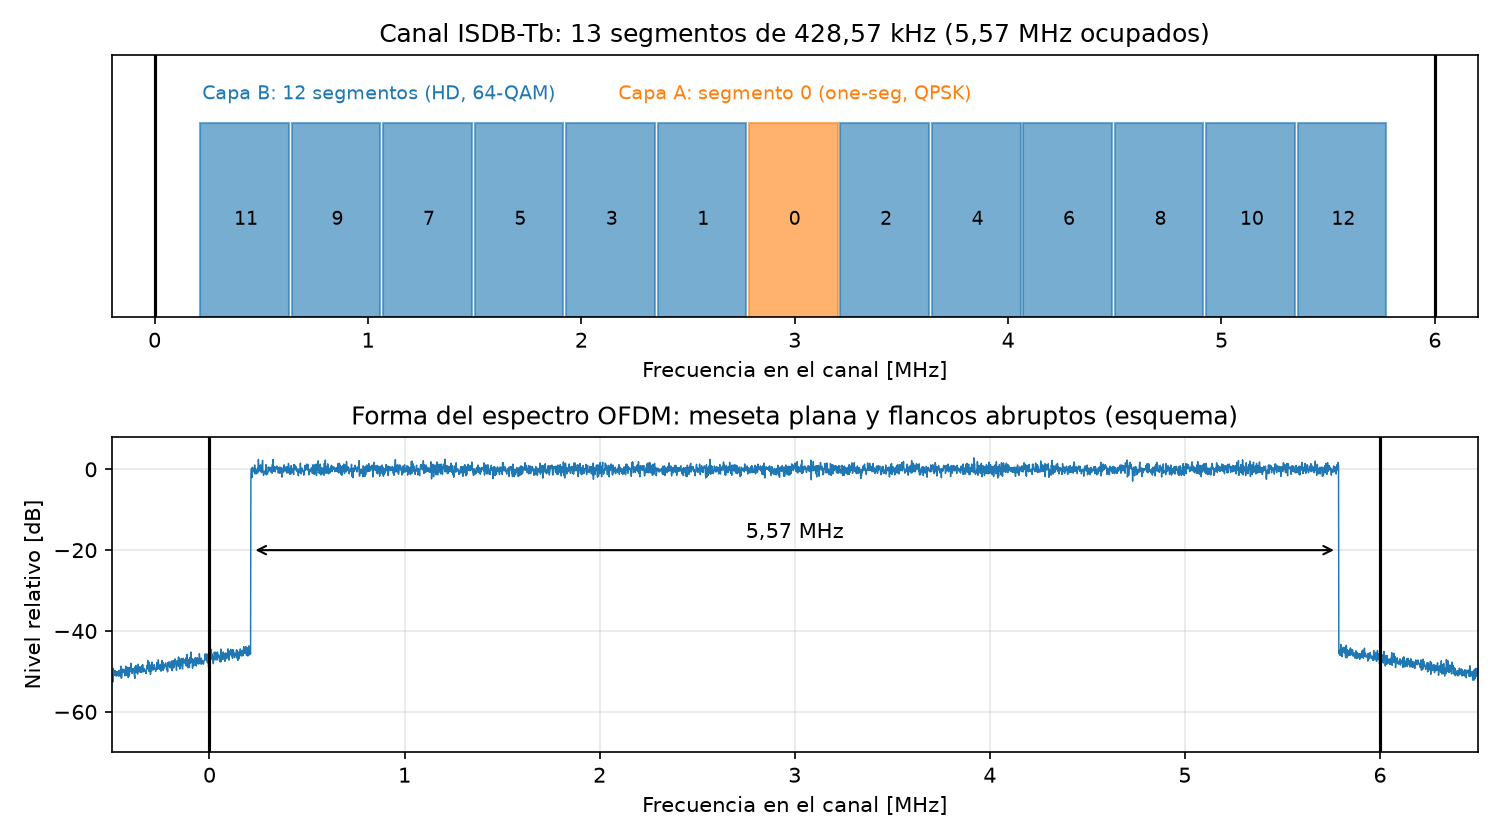
\includegraphics[width=\textwidth]{teoria/isdbtb_segmentos.png}
    \caption{Organización del canal ISDB-Tb en 13 segmentos con la configuración típica de dos capas, y forma del espectro OFDM (esquemas propios).}
    \label{fig:isdbtb_segmentos}
\end{figure}

\subsection{Distintos servicios en un mismo canal}
Los 13 segmentos se agrupan en hasta tres capas jerárquicas (A, B y C), cada una con su propia modulación, tasa de código del código convolucional interno ($1/2$, $2/3$, $3/4$, $5/6$ o $7/8$) y profundidad de entrelazado temporal. Las modulaciones posibles son DQPSK, QPSK, 16-QAM y 64-QAM. Cada capa transporta su propio flujo de transporte, con uno o varios programas.

La configuración más usada en la TDA es de dos capas:
\begin{itemize}
    \item \underline{Capa A:} el segmento central (\textit{one-seg}), con QPSK y tasa de código $2/3$, para receptores portátiles y teléfonos.
    \item \underline{Capa B:} los otros 12 segmentos, con 64-QAM y tasa $3/4$, para un programa en alta definición o varios en definición estándar para recepción fija.
\end{itemize}
Así, una sola emisora transmite al mismo tiempo, en la misma frecuencia, el programa en HD y su versión para dispositivos móviles. Otras combinaciones permiten, por ejemplo, tres capas o varios programas SD en la capa B (multiprogramación).

\subsection{Recepción fija y móvil}
\begin{itemize}
    \item \underline{Recepción fija:} con antena exterior directiva, a una altura de unos $10 \, [m]$, el receptor tiene buena relación señal a ruido y un canal estable. Se pueden usar modulaciones densas, como 64-QAM con tasa de código alta, que maximizan la capacidad.
    \item \underline{Recepción móvil y portátil:} antenas pequeñas a nivel del suelo, dentro de edificios o en vehículos. El receptor tiene menor señal, multitrayecto intenso y variaciones rápidas del canal por efecto Doppler, y necesita modulaciones robustas, como QPSK con tasa $1/2$ o $2/3$, entrelazado temporal largo y, a veces, un modo con menos subportadoras.
\end{itemize}
El \textit{one-seg} es la solución de ISDB para la recepción móvil: al ocupar solo $430 \, [kHz]$, el receptor consume menos y puede integrarse en un teléfono.

\subsection{Configuración, capacidad y robustez}
La capacidad de una capa es proporcional a la cantidad de segmentos, a los bits por símbolo, a la tasa de código y al factor de guarda. Para un segmento en el modo 1, con 96 subportadoras de datos:
\begin{equation}
    R_{seg} = \frac{96 \cdot \log_2 M \cdot r \cdot \frac{188}{204}}{T_u\,(1 + T_g/T_u)}
    \label{eq:tasa_segmento}
\end{equation}
El resultado no depende del modo, porque al duplicar las subportadoras se duplica la duración del símbolo. Por ejemplo, con 64-QAM, $r = 3/4$ e intervalo de guarda $1/8$:
\begin{equation}
    R_{seg} = \frac{96 \cdot 6 \cdot 0{,}75 \cdot 0{,}922}{252 \, [\mu s] \cdot 1{,}125} = 1{,}40 \, [Mbps]
\end{equation}
y los 12 segmentos de la capa B dan $16{,}8 \, [Mbps]$, suficientes para un programa HD y uno SD en H.264. La capa A con QPSK y $r = 2/3$ aporta $0{,}42 \, [Mbps]$. Según la configuración, el canal completo ofrece entre $3{,}65 \, [Mbps]$ (DQPSK, $r = 1/2$, guarda $1/4$) y $23{,}2 \, [Mbps]$ (64-QAM, $r = 7/8$, guarda $1/32$).

Cada aumento de capacidad se paga con robustez: pasar de QPSK a 64-QAM triplica los bits por símbolo, pero exige unos $12 \, [dB]$ más de relación señal a ruido. Una tasa de código más alta tiene menos redundancia para corregir errores, y un intervalo de guarda más corto tolera ecos más cortos y limita el tamaño de una SFN. La configuración se elige según el servicio y el área de cobertura que se quiere alcanzar.

\section{ISDB-Tb sobre cable}
\label{sec:isdbtb_cable}

La propuesta es distribuir por una red de cable canales modulados en ISDB-Tb, la misma norma de la TDA, en lugar de canales analógicos PAL-N o digitales DVB-C. Cada canal de $6 \, [MHz]$ de la grilla de cable lleva una señal OFDM idéntica a la de una emisora terrestre, con uno o varios programas. Se usa sobre redes coaxiales o HFC de $75 \, [\Omega]$, tanto en cableoperadores como en instalaciones cerradas de edificios, hoteles o clínicas, y también puede entregarse por RF Overlay en una red FTTH (\autoref{sec:rf_overlay}).

La ventaja principal es que los televisores vendidos en Argentina en los últimos años traen un sintonizador ISDB-Tb incorporado, porque es la norma de la TDA. Al recibir los canales en esa norma, el televisor los sintoniza y los decodifica directamente, sin decodificador externo, y el operador puede reemplazar los canales analógicos por canales digitales en alta definición sin instalar un decodificador por televisor. Además, en un canal de $6 \, [MHz]$ entran varios programas digitales donde antes había uno analógico, lo que libera espectro para DOCSIS.

\subsection{Equipos}
En la cabecera, los receptores toman las señales de origen (satélite, fibra o IP), los codificadores H.264 comprimen las que llegan sin comprimir o en otro formato, y un multiplexor-modulador ISDB-Tb arma los flujos de transporte y genera las portadoras OFDM en los canales elegidos; un combinador de RF las suma al resto de la grilla. La red es la misma red de cable, con sus amplificadores y derivadores, en la que hay que respetar los niveles y la planicidad de la respuesta, porque una inclinación del espectro dentro del canal deja algunas subportadoras con menor relación señal a ruido. En el abonado alcanza con un televisor con sintonizador ISDB-Tb conectado al coaxial.

\subsection{Compatibilidad con los receptores}
Como la señal cumple la norma terrestre, los fabricantes declaran compatibilidad con cualquier receptor ISDB-Tb. VideoSwitch indica que su equipo genera las portadoras según ARIB STD-B31 y ABNT NBR 15601 y que el uso de ISDB-Tb en redes cableadas ``permite la transmisión de televisión digital HD sin necesidad de agregar receptores externos al TV'' \cite{videoswitch_dmm}. Del análisis propio, no de la documentación del fabricante, surgen dos condiciones: el televisor debe poder sintonizar las frecuencias que use el operador, ya que algunos receptores podrían explorar sólo los canales UHF 21 a 51 de la TDA, y como los televisores comunes no tienen módulo de acceso condicional, los programas deben distribuirse sin cifrar.

\subsection{Ejemplo de solución comercial: VideoSwitch DMM-3100}
VideoSwitch, empresa argentina de Buenos Aires, fabrica el modulador-multiplexor DMM-3100, ``ISDB-Tb Over Cable'', destinado a cableoperadores e instalaciones cerradas como hoteles y sanatorios (\autoref{tab:dmm3100}). Según la prensa del sector, la empresa desarrolló esta tecnología para ofrecer HD y liberar ancho de banda en la red de cable, y su primera venta fue a Telecom \cite{prensario_videoswitch}. Otros fabricantes ofrecen soluciones equivalentes, como el módulo Luminato ISDB-T de Teleste \cite{teleste_isdbt}.

\begin{table}[H]
    \centering
    \caption{Características del VideoSwitch DMM-3100 según la hoja de datos del fabricante \cite{videoswitch_dmm}.}
    \label{tab:dmm3100}
    \begin{tabular}{p{4cm} p{10.2cm}}
        \toprule
        \textbf{Característica} & \textbf{Valor declarado} \\
        \midrule
        Modulación & COFDM según ARIB STD-B31 y ABNT NBR 15601 \\
        Portadoras y salidas & Hasta 8 portadoras de $6 \, [MHz]$, en 2 salidas de $75 \, [\Omega]$ con hasta 4 portadoras adyacentes cada una, ágiles de $50$ a $863 \, [MHz]$ \\
        Potencia de salida & De $-18$ a $+3 \, [dBm]$ \\
        Entradas & 4 ASI y 1 GbE (UDP/IP unicast o multicast) \\
        Multiplexación & Hasta 32 servicios por portadora, con generación automática de tablas PSI/SI \\
        Formato & 1 unidad de rack de 19", fuentes redundantes, monitoreo por SNMP \\
        \bottomrule
    \end{tabular}
\end{table}

No se encontró una norma específica de ISDB-Tb sobre cable: la propuesta aplica la norma terrestre al medio cableado.

\subsection{Comparación con DVB-C}
En un canal de $6 \, [MHz]$, ISDB-Tb llega como máximo a $23{,}2 \, [Mbps]$, contra $38{,}5 \, [Mbps]$ de DVB-C con 256-QAM (\autoref{sec:dvbc}), porque las herramientas de robustez de OFDM (intervalo de guarda, pilotos y codificación convolucional) consumen capacidad y no son necesarias en el cable. A cambio, ISDB-Tb funciona con el parque de televisores existente, mientras que DVB-C requiere decodificadores salvo en los televisores que lo incluyen. Para un cableoperador argentino que quiere digitalizar los canales básicos sin entregar decodificadores, la compatibilidad pesa más que la eficiencia espectral.

\newpage
\section{Conclusiones}
\label{sec:conclusiones}

\subsection{Principales resultados}
\begin{itemize}
    \item \underline{AM:} se identificaron Cadena 3 ($700 \, [kHz]$) y Radio Mitre ($810 \, [kHz]$), con portadoras de unos $-101$ y $-102 \, [dBm]$, apenas $3 \, [dB]$ por encima del piso de ruido. Con la antena de varillas, pensada para VHF, las bandas laterales quedaron ocultas, por lo que el ancho de banda ocupado y la máxima frecuencia modulante sólo se analizaron en forma teórica (como máximo $10 \, [kHz]$ y unos $5 \, [kHz]$, según la canalización). Con el generador, la modulante cuadrada produjo el peine de bandas laterales en las armónicas impares, separadas $2 f_m = 20 \, [kHz]$, que predice su serie de Fourier; con la senoidal, el RBW de $9 \, [kHz]$ no permitió resolver las bandas laterales a $10 \, [kHz]$ de la portadora, y el índice de modulación no pudo verificarse.
    \item \underline{FM:} se distinguieron alrededor de una docena de emisoras, con niveles de $-90$ a $-65 \, [dBm]$. La emisora de $88{,}9 \, [MHz]$ ocupó unos $220 \, [kHz]$ con el criterio de $-26 \, [dB]$: algo más que la separación de $200 \, [kHz]$ entre canales y entre los valores de Carson para una emisión monofónica ($180 \, [kHz]$) y una estéreo ($256 \, [kHz]$). Junto a ella se observó una emisora en el canal adyacente, con los flancos de ambas casi en contacto cerca del piso de ruido. La captura en barrido simple de la emisora de $102{,}3 \, [MHz]$ mostró que el espectro instantáneo de una FM con programa cambia en cada barrido.
    \item \underline{Televisión analógica:} se recibieron los canales 8, 10 y 12, con los canales intermedios 9 y 11 libres, como prevé la planificación. En los canales 10 y 12 se ubicaron la portadora de video, a $1{,}25 \, [MHz]$ del borde inferior, y la de audio, $4{,}5 \, [MHz]$ más arriba y unos $10 \, [dB]$ por debajo; en el canal 12 se distinguió además la subportadora de color. Las bandas laterales de video quedaron bajo el piso de ruido, por lo que su ancho de banda no pudo medirse.
    \item \underline{TDA:} se observó el canal 27 como una meseta de unos $5{,}5 \, [MHz]$, coherente con los $5{,}57 \, [MHz]$ de la señal ISDB-Tb, sin portadora destacada y con una potencia de canal estimada en unos $-61 \, [dBm]$, unos $11 \, [dB]$ por encima del piso de ruido del analizador. No se realizó la prueba con un televisor, por lo que no se compararon las señales observadas con los servicios decodificados.
    \item \underline{Niveles:} la conversión entre dBm y dBµV depende de la impedancia ($+107{,}0 \, [dB]$ en $50 \, [\Omega]$ y $+108{,}8 \, [dB]$ en $75 \, [\Omega]$), mientras que los niveles en dBc no dependen de ella. En el ejercicio, una banda lateral de $-40 \, [dBc]$ corresponde a un índice de modulación del $2 \,\text{\%}$.
    \item \underline{Distribución por cable y fibra:}
    \begin{itemize}
        \item DVB-C aprovecha la alta relación señal a ruido del cable con QAM de portadora única, y transporta unos $38 \, [Mbps]$ por canal de $6 \, [MHz]$ con 256-QAM.
        \item DOCSIS convierte la red HFC en una red de datos bidireccional, y es la base del acceso a Internet y de la migración del video a IP.
        \item El RF Overlay lleva todo el espectro de una red de cable en $1.550 \, [nm]$ sobre la ODN de una red FTTH, sin consumir capacidad de datos y sin decodificadores, a costa de equipamiento óptico de video y sin interactividad. La IPTV, en cambio, integra el video en la red de datos.
        \item ISDB-Tb usa OFDM en 13 segmentos y capas jerárquicas, que permiten combinar en un canal servicios fijos en HD y servicios móviles.
        \item ISDB-Tb sobre cable aprovecha que los televisores argentinos ya traen sintonizador ISDB-Tb para digitalizar las redes de cable sin decodificadores, a cambio de una capacidad por canal menor que la de DVB-C.
    \end{itemize}
\end{itemize}

\subsection{Dificultades y limitaciones de las mediciones}
\begin{itemize}
    \item \underline{Antena:} la antena interior de varillas telescópicas es adecuada para VHF, pero en la banda de AM es eléctricamente muy corta, lo que dejó a las emisoras de AM apenas por encima del piso de ruido.
    \item \underline{Piso de ruido del analizador:} en torno a $-100 \, [dBm]$, ocultó las bandas laterales de AM, las de video de la televisión analógica y, posiblemente, otros canales digitales de bajo nivel.
    \item \underline{Resolución del instrumento:} el RBW de $9 \, [kHz]$ es comparable con el canal de AM y con la separación de las bandas laterales de la señal generada, y no las resuelve; un RBW menor hace más lento el barrido.
    \item \underline{Señales de programa:} su espectro varía todo el tiempo, por lo que los anchos de banda medidos dependen del tiempo de observación, de la retención de máximos y del criterio de nivel adoptado.
    \item \underline{Lectura de los valores:} los niveles y frecuencias se leyeron sobre la grilla de fotografías de la pantalla, por lo que son aproximados; con los marcadores del analizador se habría obtenido mayor precisión.
    \item \underline{Impedancia:} el analizador mide en $50 \, [\Omega]$ y las antenas y redes de televisión son de $75 \, [\Omega]$. La desadaptación o el adaptador agregan un error o una atenuación que hay que considerar.
    \item \underline{Equipamiento:} no se dispuso de un televisor o receptor ISDB-Tb, por lo que no se pudo comprobar la recepción de la TDA.
\end{itemize}


\newpage
\printbibliography[heading=bibintoc, title={Fuentes consultadas}]
\end{document}
